\restoregeometry
\section{专业数学培养}

 {\itshapeCJK
  数学是研究现代科学与技术的基本语言,力学更是工科之中与数学联系较为紧密的学科。掌握足够的数学知识是十分必要的,其意义不仅仅是为了应付考试,更在于掌握数学知识有助于准确地把握力学问题的本质,以及快速入门未曾研究过的专业问题,等等。学好力学的核心,除了培养力学专业的思维方式与直觉,最重要的便是要学好数学知识了。

  不过,学习任何一门学科都是需要付出很多精力的,特别是数学是一门对抽象思维能力要求较高的学科,学习起来的确有一定难度。所以我们最关心的问题自然是:如何学好数学?这其实是一个很大的问题,我们这里只能根据从笔者有限的经历,对学习的总体方法论和知识树作一简介,姑且算是给读者提供大致的理论指导。而读者则需要根据自身实践,对我们提供的指导思想做适合自己的调整,找到最适合自己的学习节奏。

  此外,力学的学习与数学的学习具有一定的相似性,有些方法是相通的,但我们着重介绍基础数学知识,对力学专业内容不做展开,还请读者在后续学习中自行体会与摸索。
 }

~\\

\subsection{总体方法论}

\subsubsection{培养自学能力}

大学教育与中学阶段的最显著的区别是,授课教师不会像以前一样手把手地教,把所有的知识点都嚼碎之后喂给我们。实际上,大学设置课程的质量参差不齐,如果只是一味地跟着授课教师亦步亦趋,往往是学不到多少东西的。同时,在以后的研究、工作之中,很多事情也都需要自己去想办法解决。所以培养自学能力就十分重要了。那么,如何培养自学能力?

\paragraph{兴趣是最好的老师}

作为一名理工科学生,在学习过程中会用到很多数学。微积分、线性代数等等不一而足,然而对于力学系的同学来说,计算能力和建模应用是首位的,逻辑上的推理以及严格性的证明往往是被我们作为学习数学辅助手段来使用的。

力学系的同学使用数学工具的过程中,常常会对自己使用的数学工具产生疑问,这样做是否是合理的?为什么会是这样?为什么有的地方满足交换律,到了别的地方就不满足了?同样是两个方程确定的偏导数,为什么在表达顺序上会出现异常的规律?$x$ 和 $y$,究竟在哪里等价,在哪里又不等价?深入的思考带来的疑问,驱使着我们去发现未知的数学规律,而在这个过程又会带来极大的愉悦和满足。从工科的角度学习数学就是这样一个过程,从使用中产生疑问,在解答疑问的过程中产生新的想法。大学毕业以后,有些专业课有可能以后很难再接触到,真正珍贵的是自己独立思考的过程,和灵光一现,再到解决疑问的愉悦感。

在大学里,建立良性的循环是非常有必要的。什么是良性的循环?不妨先看看什么是恶性的循环。假如你有一天熬夜到很晚,第二天跟不上老师,下课后作业不会,费尽心思搞懂又是深夜。在这个过程中一点点磨灭掉自信心,从此开始摆烂,直到挂科,退学等等事情的发生。规律的作息是保证良好心态,形成良性循环很重要的一部分。而良性循环就刚好相反,比如学习——兴趣——思考——学习的过程,这样的循环对于坚持学习是非常重要的,学习的开始往往是从兴趣开始的,这也是为什么兴趣是最好的老师。

\paragraph{资料与信息检索}

\begin{enumerate}
    \item 善用图书馆。如果将图书馆只是当作自习室,那实在是暴殄天物。对于一个大学生来说,图书馆有着最直接也最好用的海量图书资源。你可以在图书馆借到大量的、侧重点各不相同的同一类书籍。有些大学的图书馆会有许多国外的或者国内已经绝版的、甚至是独一无二的优质资料。不夸张的说,图书馆至少能够满足一般人在本科阶段大多数的资料需求。同时,善用图书馆的检索功能,掌握书籍的检索规律,还能锻炼资料检索的能力。
    \item 电子资源的检索。Zlib、知网、Sci-Hub、学校图书馆的线上借阅、各种不知名的小网站、百度网盘等等都藏有许多资源,这种资源检索往往需要对所研究的领域有一定了解。在入门阶段,不妨应用百度、知乎、Google、CSDN等检索平台,对于某些领域来说能够满足快速入门,获得一个初步印象的需求。
          关于更多的具体的数学检索平台,可参见USTC基础数学修课指南。
    \item 充分调动人脉资源。很多时候,我们缺少的往往是获得关键信息、资料的途径,这些内容不是通过阅读已有书籍或电子资料就能获得的。这时候,要积极地向身边或线上了解相关领域的朋友请教,他们手中的资料、他们对于该领域的见解,都是相当宝贵的信息,这要比自己探索方便快捷得多。但是,如果有志于独立研究,也不要过分依赖于他人的帮助,因为总有一天会面临无人可问的情形。
\end{enumerate}

\paragraph{正确处理习题,形成自我评估}

对于习题的争论,历来分成两派,一派主张“题海战术”,另一派与之相反。究竟应该选择哪一种,取决于学习动机。

对于应试来说,“题海战术”确实是行之有效的方案。但对于一般性的学习,我们不建议直接捧着习题集做,却也不是少做题。在反对“题海战术”的思潮中,也有另一种极端,即动笔很少,这也是不可以的。题必须要做,只是最好要有选择性地做、精做。做题的主要目的有两个:一是通过操作实例,积累经验与直觉,所以像《吉米多维奇》这样习题重复度过高的参考书并不值得大家花时间去大做特做;二是检验学习程度,判断目前的水平是否可以继续深入学习,只有打牢基础才能钻研更深入的知识,前置知识掌握得不牢固,学习后续知识就容易出现困难。

如何做题也是有讲究的。首先,尽量选择有参考答案,最好是有详细解答步骤的题目去做。其次,在做题时,独立思考是很重要的,但也不要受“独立思考”这种说法的束缚,题目中某个关键步骤如果想了很长时间也没想出来,就应该直接去看答案了。我们的目的是掌握方法,把答案看懂(而不是囫囵吞枣)当然能够掌握方法,没必要有什么心理负担,我们如今所学的知识都是前人经过数十年、数百年浓缩而成的,把所有细节全都背下来,既是不现实的,也是没必要的。

\paragraph{快速入门学科,不必万事俱备}

在学习和科研的过程中,我们常常有快速入门一个学科/领域的需要。要想快速入门一门学科,最好还是直接看问题,从问题下手往往是最快的,因为这时有足够的动机。不必管解答,无论能否看懂,起码都会先有一个印象,以及自己思考的过程,这样就可以算得上入门了,入门之后再去考虑其中的细节问题。

比较忌讳的是为了一个领域/专业课,去大学特学前置知识。一来这样效率低;二来准备得完全充分也是不现实的,在学习和研究的过程中经常会出现新的概念,现用现学才是常态;三来是不同专业的侧重点不完全一样,如果学了某样“前置知识”,到最后发现在专业课的实际应用中并没有用到那么多知识,就有点得不偿失了。

此外,快速入门的另一个前提是要有广泛的知识储备,也就是说在一定程度上当一个“名词党”是有好处的。不管怎么说,知道有一个名词比不知道强,在前期调研时至少有一个大致方向。第一次接触某一个名词时,不一定要对其有多么深入的理解,哪怕仅仅是形式上接受它也未尝不可。

\paragraph{学数学是一个积累的过程}

很多人可能会认为,理工科类型知识的学习只要捋顺逻辑即可,无需进行记忆。事实并非如此,倒不是说我们需要去背公式、记习题,而是要积累观点、思想方法和典型例子。“数学成熟度”是一个比较玄学的指标,看不懂书的时候,可能有人会对我们说:“这是数学成熟度不够导致的”。“数学成熟度”大概指的就是我们习惯一套数学语言的程度,我们在数学上做积累的目的就是提高“数学成熟度”。

如何提高“数学成熟度”呢?凡事没有捷径,唯一的捷径就是抛开杂念去做。数学的学习,分为输入和产出的过程。看书、做题、上课是输入,与人交流、整理笔记、编写讲义、写小论文等是输出的过程。数学思维的建立不是技巧的堆砌,而是积累大量的数学观点和思维方式,能说出定理和定理、学科与学科之间的关系。循序渐近,多看、多写、多想,才能逐渐提高“数学成熟度”。这是一个或长或短的积累的过程,不必急于求成,踏实去学才能厚积薄发。

\paragraph{一些学习方法}

在学习过程中,还有一些具体的方法:

一定要充分发挥主观能动性,我们的目的是学知识,不是折磨自己。这意味着可以先通读学习材料,先对知识形成一个整体印象,遇到不懂的一个点可以选择性地跳过,待通读若干遍之后,再精读,去认真考察其中的细节。这也是一般阅读文献应该采用的思路。

抄书是自学的有效方法。它可以是选择性地摘录重点,也可以是事无巨细地誊写,抑或是学习一遍后的总结、归纳。这种方法看似笨重无比,实际上是能稳定获得较大收益的办法,抄书能辅助你集中注意力,完成构建知识体系的过程。

若是比较关心数学的力学应用,则不必限于技术性细节,更多地关注计算与应用。可以选择性地忽略一些严谨的证明,暂时接受一项结论,在具有一定理解的前提下考虑如何去计算和应用,通过不断地计算和应用反过来加深对概念的理解,这既包括对数学概念本身的理解,也包括概念及相关的计算方法可以被应用在哪些物理和力学模型下,在有进一步需要的情况下,可以考虑花些时间仔细地研读证明过程。

若是出于兴趣,或是为了学习一些高级的数学理论和工具,请一定打好前置知识的基础,关心问题的处理思想与方法,关键性的推理与证明都不要放过。很多进阶的概念和方法是从比较基本的问题中提炼、概括出来的,对基本背景问题有足够的了解,能更好地理解提出某项概念或定理的动机,以及了解其研究思路,处理一些问题时能有一个大致的思路。

\subsubsection{形成认识与对待数学的观点}

之所以单独开设这一个板块,是因为笔者发现即使到了本科毕业的时候,仍然有许多专业内的同学没法分清数学和物理/力学之间的区别。这源自于我们中学阶段对数学基础的忽视,而只是简单归纳“性质”、“应用”造成的恶果,如果延续这种“一叶障目,不见泰山”式的思维进行学习,是走不长远的。很多人学了数年数学和物理,只能看到“数学和物理当中都有很多定理、公式”、“都需要做大量计算”,却难以分辨出二者之间除了研究对象以外的区别,只是觉得数学似乎更抽象一点,物理/力学更实际一点,实际上这是浅显的、片面的。

最重要的区别在于,数学不是自然科学,而是形式科学,而物理/力学都是自然科学。自然科学是一门以观察和实验的经验证据为基础,对自然现象进行描述、理解和预测的科学分支,就是说自然科学要取之于实践,终究也要用之于实践。形式科学并不关心真实世界与理论之间的联系,而关注以定义和规律为基础的形式系统的性质。

数学作为形式科学的属性决定了,在数学当中,只要推理是正确的,那么得到的结果就一定是正确的,不存在任何更改的余地,一旦需要修正,一定是推理出现问题,或者需要相应修改推理的前提。而在自然科学中,所有理论都是通过观察、归纳,总结出基本定律之后获得或再推理获得的,观测和归纳出现问题,都可能导致理论的修正。同时,数学也可以作为一种语言对自然科学进行定量描述,构建数学模型对实际问题加以研究,正是这一原因容易使人们看不清数学与自然科学之间的关系。

时常有人对数学发出诘难:“数学有什么用?”,然而数学作为形式科学本就不必考虑实用性,以及现实世界是什么样子的,它可以是纯粹的思维游戏,这无可非议。可是,数学又不能完全脱离实际。这话看起来有些矛盾,但一切抽象的知识和问题最初都一定来源于实践,只是经过不断地归纳、总结、抽象、一般化的过程中,我们可能已经看不出问题原来的模样。

不过作为力学专业的学生,我们更多地是把数学作为描述力学问题的语言与解决力学问题的工具。如果拿作战做一个比喻,我们的力学原理和直觉就像是战略与战术思想,指引我们的研究方向,而数学就像是支持作战的后勤保障,支持着研究进行以及这场研究能够走多远。

抽象也好,实用也罢,研究抽象数学理论和研究数学理论与现实情况之间对应关系的数学家都应该得到我们的尊重,他们从事的是人类头脑所能进行的最伟大、最艰深的活动之一。

\subsubsection{正确处理数学与力学专业的关系}

\paragraph{注意学习数学的动机}

在确认学习之前,一定要明确学习动机。学习数学应当以力学专业课程为导向,兴趣爱好为辅,无需过早地接触过于抽象的数学。我们当然支持出于兴趣学习一些高级的数学工具,而且这也是有好处的,但是一定要避免在这个过程中形成眼高手低、浮于表面的坏习惯。

我们指出,所谓高级工具本质上更接近对“相对初级”的理论的归纳、抽象、推广,有些高级工具需要学习到足够深入之后才能拿来解决一些问题,这对于力学学科来说的代价很大,务必做好取舍。也有些高级工具压根就不是为了解决现实问题服务的,或者说至少不是为了你感兴趣的领域准备的,这时也需要考虑清楚学习成本。

再者,务必端正深入学习的动机。中学阶段的应试教育培养出了一种奇怪的思潮,即所谓“应用高级数学工具对初级问题进行‘降维打击’”。经验表明,高级数学工具往往并不会直接产生“降维打击”的效果,它起到的通常是提供思路的作用,甚至可能不起作用,换句话说,通过高级工具实现“降维打击”的收益至少不明显大于打好基础的收益,“降维打击”并不是高级工具应有的作用。熟悉了高级工具之后,应该做的是去了解更广泛的数学、应用知识,在反复使用中熟悉、理解、内化,将“高级工具”变成你的“初级工具”,这才是“高级工具”正确的打开方式。

另外,如果出于应急所需,例如一门专业课要用到某样数学工具,这时也不建议直接去找一本数学理论性很强的书去看。因为数学方向与专业所需的关注点可能并不一样,这样不仅见效慢,而且更可能打击自信心,为学习徒增障碍。更好的做法是边学专业内容边补数学工具,以及找一些有附录讲解这些工具的同类书籍,在有了基础知识和专业知识后,如有兴趣,可以考虑再看相应的数学理论。

\paragraph{注意学习数学应该深入到什么程度}

力学学科与数学的联系是相当广泛的,乍一看学习力学需要特别多的数学,但实际上所有内容的基础都是微积分与线性代数,这是一切学习的根本与下限。出于不同的学习动机,学习的深入程度自然也是不一样的。

如果只是为了应付考试、科研,那掌握最基本的微积分和线性代数可能就足够了。但是,这时去备考或阅读文献可能会比较痛苦,因为很多数学概念是有更深厚的数学或物理/力学背景存在的,如果不能把握这一点,那么所做的工作可能会显得比较破碎、凌乱,不容易直击问题要害。

如果为了在科研中取得一定成果,或者对数学有一定兴趣,那么至少本科数学基础课都应该学好。我们后边将会介绍,本科阶段的基础数学课都是有用的,会在某些力学课程中用到,只会微积分和线代的话,就算能看懂,理解起来也会存在很大障碍。

如果为了专门处理某类问题,或者对某一数学领域兴趣浓厚,则应该广泛地参考课外学习资料。这个阶段不必限于培养方案中的设置,根据自己的需要、兴趣广泛地学习即可,但也要注意深入的程度,没有必要学习相当抽象的理论,仍然以计算和应用为主。(除非是确实对抽象的数学理论感兴趣,但若是如此,请自行平衡好时间和精力)

\paragraph{注意寻找与建立数学与力学之间的联系}

学过相应的数学后,一定不要束之高阁,而要寻找和思考这些数学工具可以用在哪些地方。知识只有在不断运用之中,才能得到深层次的理解,长时间不用自然会遗忘。具体的联系我们将在具体的数学科目中介绍。


\subsection{基础数学培养}

\begin{figure}[ht]
    \centering
    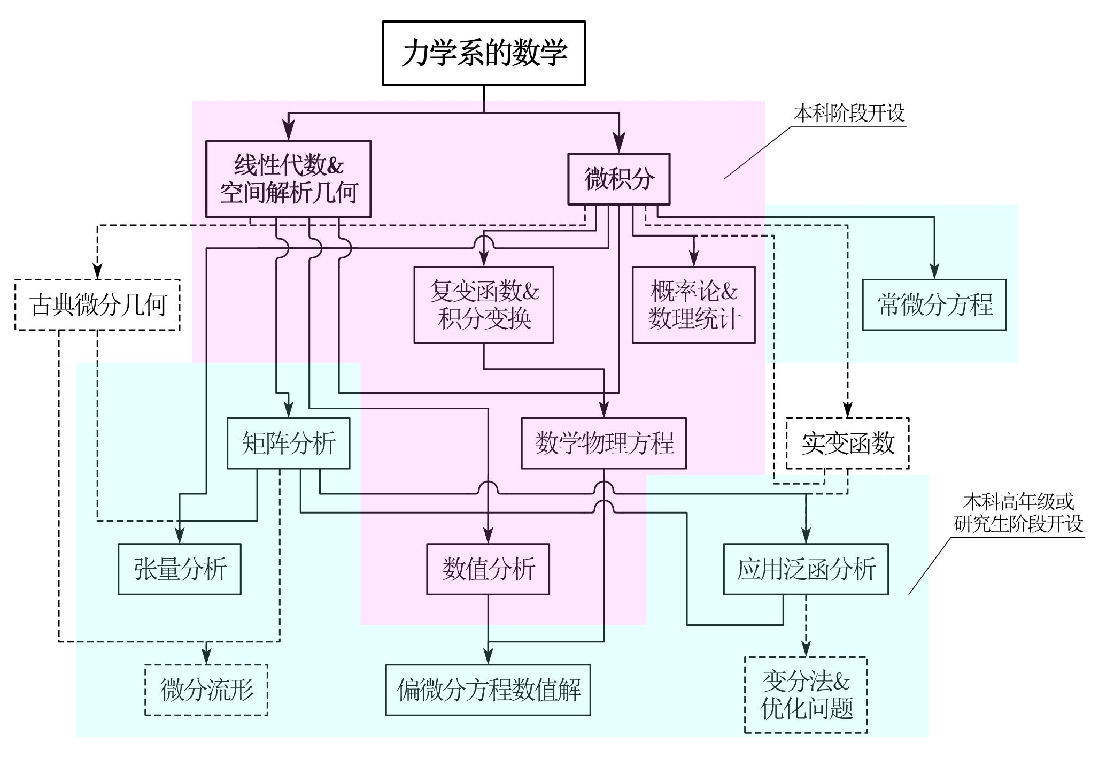
\includegraphics[width = \textwidth]{TREE.pdf}
    \caption{力学系的数学科技树}
    \label{fig:力学系的数学科技树}
\end{figure}

前一节业已提及数学的重要性,以及如何把握数学知识。本小节将介绍大学内最基本的数学知识——微积分及线性代数,以及其相关知识的基本外延。微积分和线性代数是描绘一切理工类学科知识以及进阶数学知识的基础,其重要性不言而喻,一定要给予足够重视。然而,如何有针对性地学好这两门基本数学课程,使之与日后专业知识的学习相适配,不同专业又有不同的侧重点,这里我们只勾勒力学类学生应该需要把握的大体框架。

总体而言,由于这一部分的数学课程最基础,同时也最重要,所以这一部分即使不是出于应试需要,也建议稍多做一些习题,确保对这些基础知识和处理技巧有足够的熟练度。

具体的介绍之前再次强调,我们所讲的内容不以应试为导向。

\subsubsection{微积分}

\paragraph{主体知识介绍}

微积分是研究\uwave{微分}和\uwave{积分}是数学分支。粗略地说,微分讨论的是“变化率”,积分讨论的是“累积”或“求和”。在力学上有两个经典的例子分别给出了研究微分与积分的动机:为了计算物体在运动过程中某一点$M_0$处的瞬时速度,再取一点$M$,能算出这段路程上的平均速度,当$M$足够接近$M_0$,这个平均速度就能近似描述瞬时速度,这个过程就是微分;为了计算物体在变力作用下运动过程中所做的功,先将运动轨迹分成若干段,在不同段上用分别用一个常力代替变力计算做功功,随后求和,当运动轨迹划分得足够细致时,计算的结果就近似于真实的做功大小,这个过程就是积分。

\begin{figure}
    \centering
    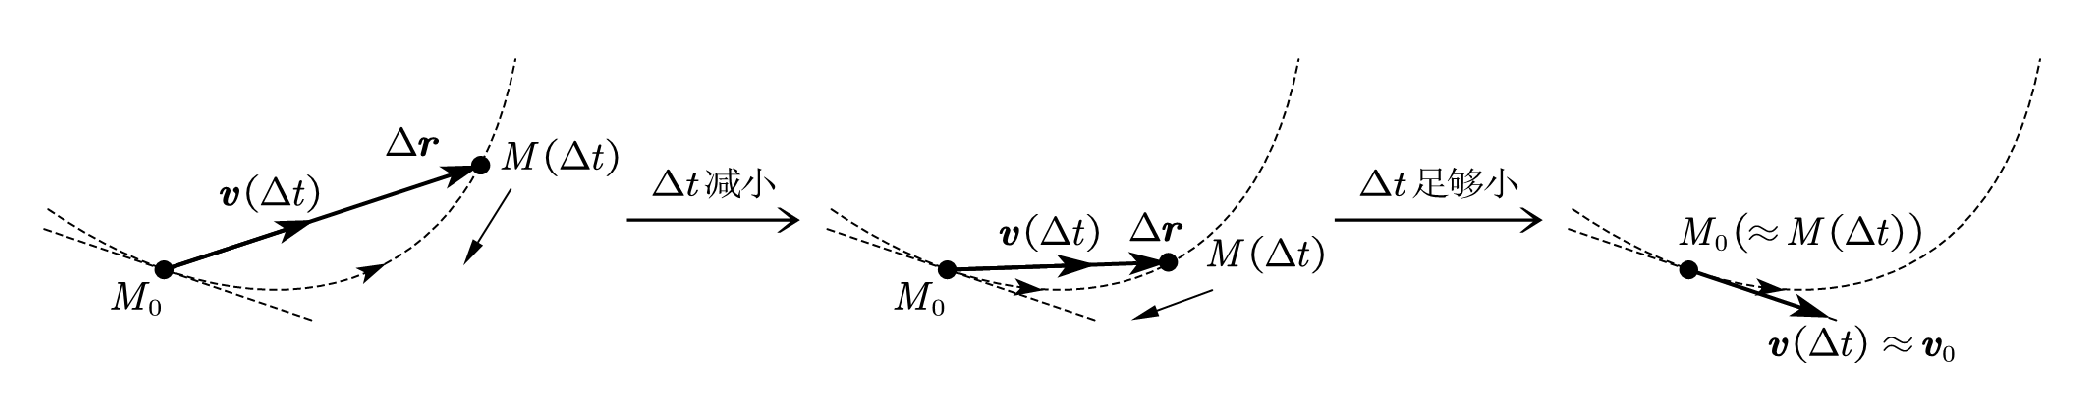
\includegraphics[width = \textwidth]{differential.pdf}
    \caption{当$M_0$运动到$M$的时间$\Delta t$足够小时,$\symbfit{v}=\dfrac{\Delta \symbfit{r}}{\Delta t}$就近似表示瞬时速度$\symbfit{v}_0$}
\end{figure}

\begin{figure}
    \centering
    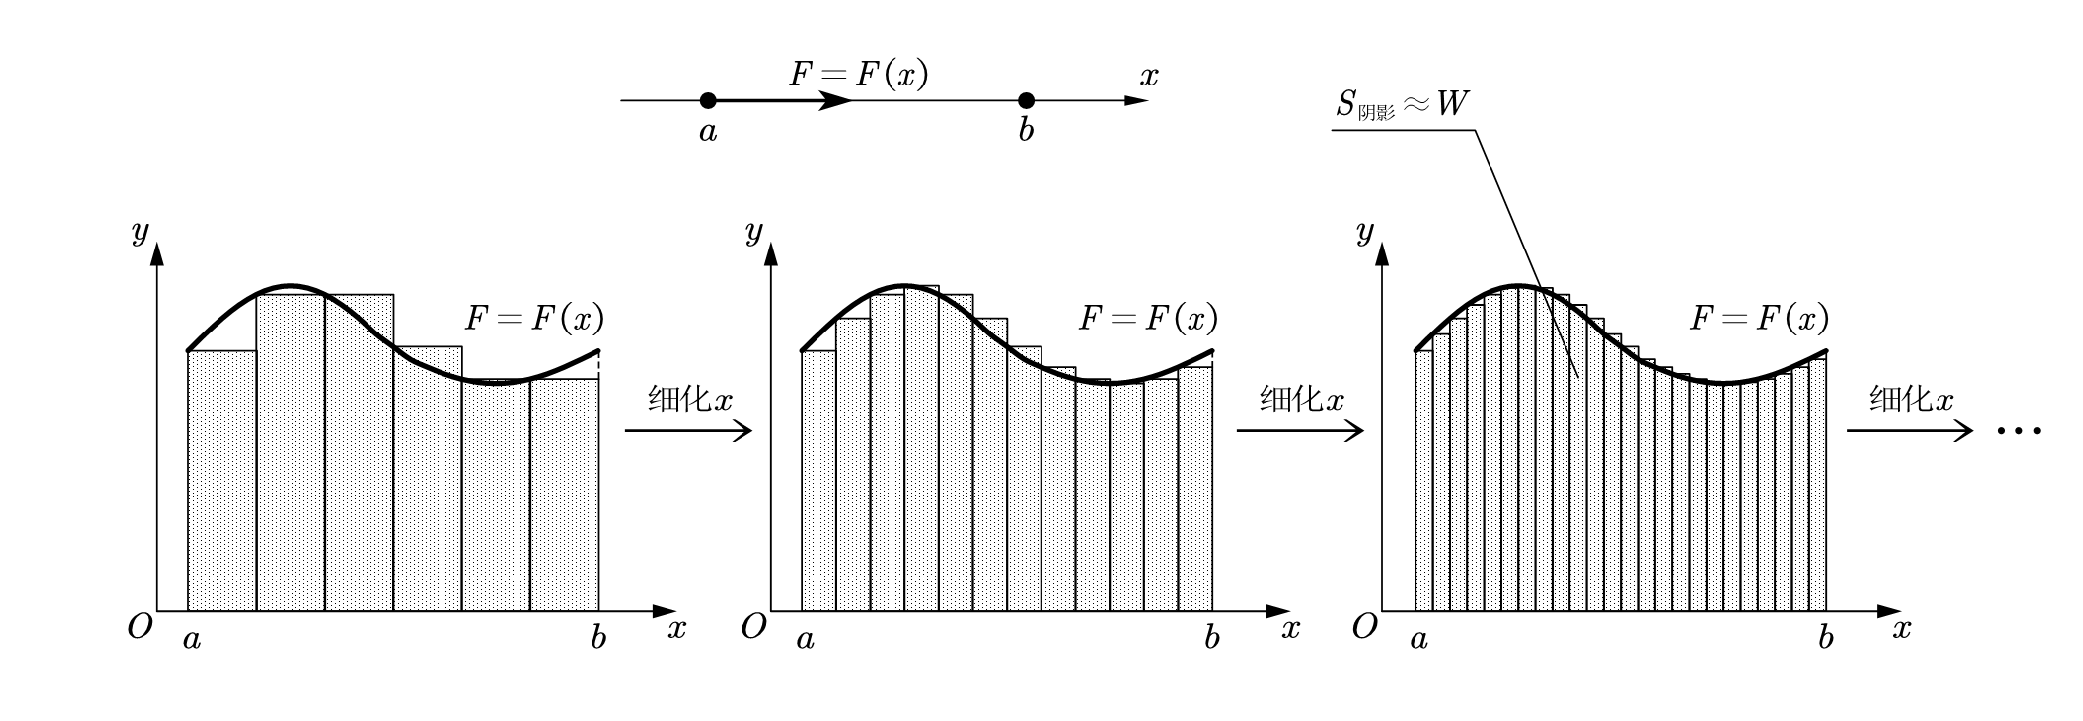
\includegraphics[width = \textwidth]{integral.pdf}
    \caption{力$F$在$x$轴上运动,从$a$到$b$所做的功}
\end{figure}

学习微积分首先要有\uwave{数列}和\uwave{函数}的概念,函数研究的是变量之间的变化关系,数列可以看成定义域离散的函数。在正式学习微积分之前,要对基本初等函数有一个了解,知道其基本性质、函数图像。

一元微积分研究的是一元函数的微分与积分,其基础是\uwave{极限}理论。

一元函数微分部分的核心技巧与内容有两块:\uwave{Taylor公式}与\uwave{微分形式不变性}。Tay-lor公式是描绘可微性足够好的函数在某点附近性质的有力工具,所以要对各种基本初等函数的Taylor公式相当熟悉,同时,它也是对“等价无穷小”这一概念的更精确的表述,能够回答“极限中函数什么时候可以做加法”的问题。微分形式不变性是能将\uwave{复合函数链导法则}、\uwave{隐函数求导}等内容串到一起的,从这里出发能将前边所学的很多东西联系起来。

\begin{figure}
    \centering
    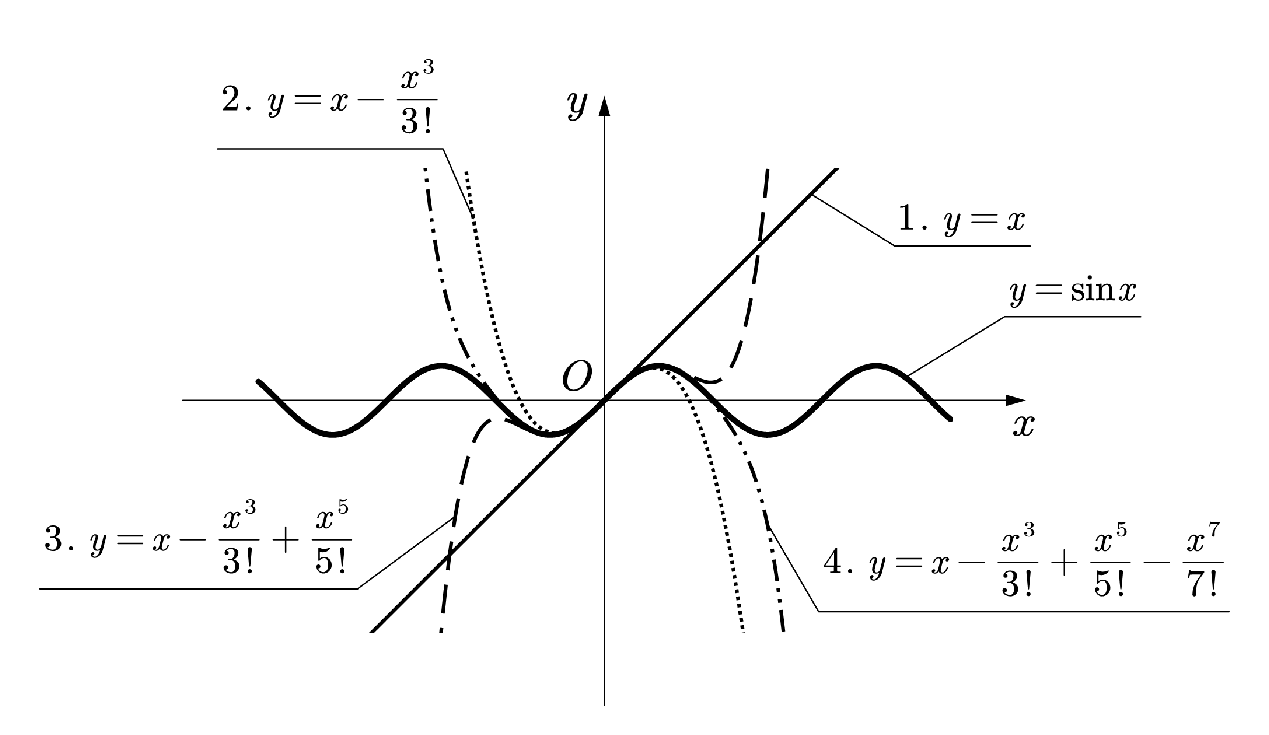
\includegraphics[scale=0.5]{Taylor.pdf}
    \caption{$y=\sin x$及其前几阶在$x=0$处的Taylor展开图像,展开项越多,在$x=0$附近越接近$y=\sin x$}
\end{figure}

关于微分需要多说一点。有些教材上对于微分的处理很模糊,较好的教材会说“微分是函数变化过程中的线性主部”,我们在此阶段,不妨就把微分看成是差分的极限。在处理一阶导数时,可以在形式上将其视为$\mathrm{d}y$与$\mathrm{d}x$的商,但是高阶导数则不行,也因此“反函数的导数是原本函数导数的倒数”这一奇怪的结论(实际上,基于微分形式不变性就能求解反函数的导数)仅能对一阶导数成立。在后续的学习中,也能看到“将微分看作某个线性空间下的基”这种观点,那是后话了,多数时候将微分看成差分的极限是够用的。

另外,涉及到无穷的讨论一定要慎重,从对有限的讨论结果直观外推的结果不一定可靠,必须要做严谨的分析!这一观念在后续课程中是很重要的。

一元函数积分比较重要的内容是\uwave{分部积分}
\[
    \int_{a}^{b} u(x)v'(x)\,\mathrm{d}x = u(x)v(x)\bigg|_a^{b} - \int_{a}^{b} u'(x)v(x)\,\mathrm{d}x
    .\]
以及\uwave{Newton-Leibniz公式}
\[
    \int_{a}^{b} F'(x)\,\mathrm{d}x = F(x)\bigg|_a^{b} = F(b)-F(a)
    .\]
不定积分运算是已知导数求原函数的过程,它与导数运算在相差一个常数意义下是互逆的。正如在正数的范围内引入减法会产生负数、在整数的范围内引入除法会产生有理数,初等函数的不定积分也会产生不属于初等函数的函数。事实上,绝大多数的初等函数的不定积分都不是初等函数,所以能够掌握一些基本的、常见的不定积分技巧,包括换元、分部积分即可。而分部积分是很重要的,这个技巧在涉及到能量的方法以及变分法中是常用的。Newton-Leibniz公式的精髓不只在于建立了函数及其导数的关联,它还建立了区间和区间边界的联系,这一点在多元积分当中的各种积分公式中也能够看到。


\begin{figwindow}[0,r,
        {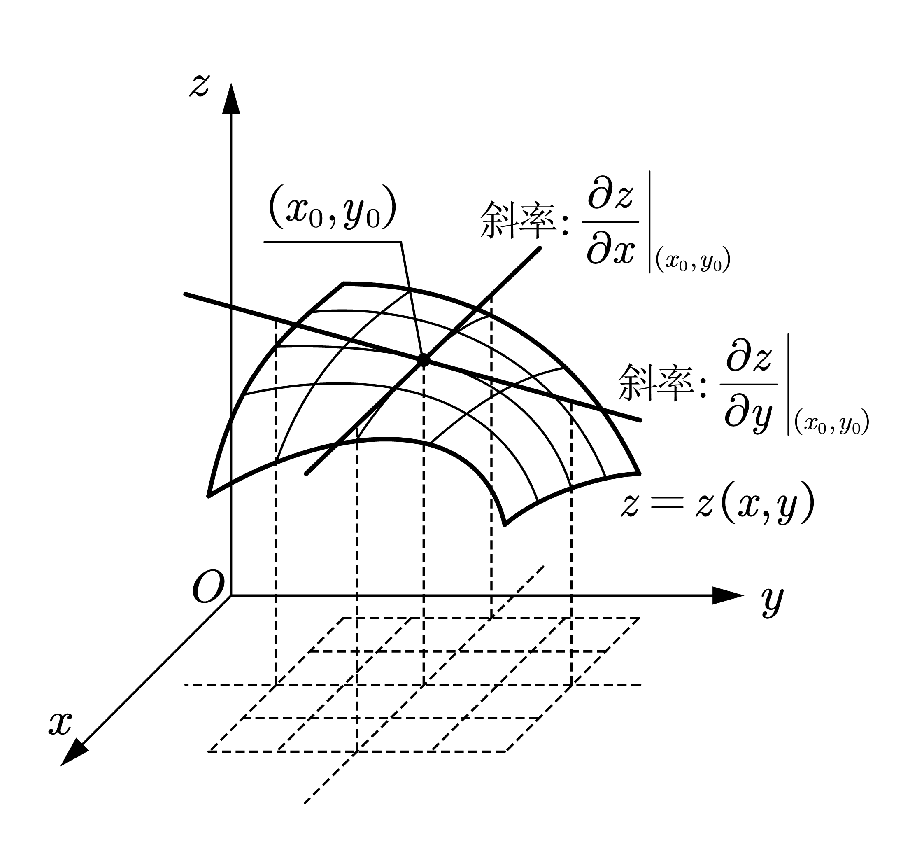
\includegraphics[width=4.5cm]{partial.pdf}},
        二元函数$z=z(x,y)$的偏导数]
    多元函数微分部分,首先要掌握$n$维欧氏空间$\mathbb{R}^n$中的诸多基本概念(拓扑性质),这些基本概念在后续学习中还会用到。最重要的概念当属\uwave{偏导数}与\uwave{全微分},偏导数只描述函数关于某一个自变量的变化情况,而全微分反映各个自变量的影响,因此全微分比偏导数要强很多。类似一元微分学部分,全微分也具有形式不变性,同时也能搞定复合函数求导以及隐函数求导。这里可能要注意不同学科的习惯不同,比如力学中,设有一个函数形式为$L=L(q(t),t)$,若要求其对时间$t$的全导数,往往会写成以下形式:
\end{figwindow}

\[
    \frac{\mathrm{d}L}{\mathrm{d}t}=\frac{\partial L}{\partial q}\frac{\mathrm{d}q}{\mathrm{d}t}+\frac{\partial L}{\partial t}
    .\]

形式上看,这种记法符合全微分形式不变性,但数学上可能记$L=f(q(t),t)$,其对$t$的全导数为

\[
    \frac{\mathrm{d}L}{\mathrm{d}t}=\frac{\partial f}{\partial q}\frac{\mathrm{d}q}{\mathrm{d}t}+\frac{\partial f}{\partial t}
    .\]

没有哪一种写法是错的,只要注意不同的习惯约定即可。多元函数微分学常用一些空间解析几何的内容,在此之前最好先学习一下相关内容,知道常见空间曲线、曲面的解析式。另外,从这里开始逐渐接触到一些涉及到\uwave{梯度场}的知识,由于数学工具限制,在这一阶段不会太过深入,知道一些关键结论和初步应用即可。

多元函数积分与场论部分,首先要熟悉基本的累次积分、二、三重积分的计算,以及不同坐标系下积分微元的关系。随后是两类曲线 / 曲面积分,第一类曲线积分主要注意选择合适的参数将弧微元转化成关于参数的一重积分,第一类曲面积分主要注意选择合适投影面将面微元转化成关于两个坐标的二重积分。第二类曲线 / 曲面积分是矢量积分,一方面注意其与第一类曲线 / 曲面积分的联系,另一方面注意\uwave{Green公式}、\uwave{Gauss公式}、\uwave{Stokes公式}\footnote{可以看到,Green公式、Gauss公式、Stokes公式与Newton-Leibniz公式类似,都将函数及其导数,以及区域及其边界联系了起来。}
\begin{gather*}
    \iint_{\sigma} \left(\frac{\partial Q}{\partial x}-\frac{\partial P}{\partial y}\right)\mathrm{d}x\,\mathrm{d}y                                                                                                                                                                                                     = \oint_{\partial \sigma} P\,\mathrm{d}x+Q\,\mathrm{d}y,                                                        \\
    \iiint_{\Omega} \left(\frac{\partial P}{\partial x}+\frac{\partial Q}{\partial y}+\frac{\partial R}{\partial z}\right)\mathrm{d}x\,\mathrm{d}y\,\mathrm{d}z                                                                                                                                                         = \oiint_{\partial \Omega} P\,\mathrm{d}y\,\mathrm{d}z+Q\,\mathrm{d}z\,\mathrm{d}x+R\,\mathrm{d}x\,\mathrm{d}y, \\
    \iint_{\Sigma} \left(\frac{\partial R}{\partial y}-\frac{\partial Q}{\partial z}\right)\mathrm{d}y\,\mathrm{d}z+\left(\frac{\partial P}{\partial z}-\frac{\partial R}{\partial x}\right)\mathrm{d}z\,\mathrm{d}x  +\left(\frac{\partial Q}{\partial x}-\frac{\partial P}{\partial y}\right)\mathrm{d}x\,\mathrm{d}y = \oint_{\partial \Sigma} P\,\mathrm{d}x+Q\,\mathrm{d}y+R\,\mathrm{d}z.
\end{gather*}

的运用。此外,此处会进一步涉及\uwave{散度场}、\uwave{旋度场}的内容,需要熟知\uwave{梯度算子}\;$\nabla$的基本计算,以及“有势无旋、有旋无源”等常用的结论。

一般的微积分教材还会有两个专题,一是\uwave{常微分方程},二是\uwave{无穷级数}。微积分课程中所讲的常微分方程是比较有限的,最重要的当属\uwave{常系数线性微分方程}和\uwave{Euler方程},我们重点关注其求解。无穷级数中最重要的是\uwave{Taylor级数}和\uwave{Fourier级数},Taylor级数部分注意运用运算规则推导常用的级数,Fourier级数部分在计算Fourier系数时,常用分部积分的技巧。

\begin{wrapfigure}{r}{5cm}
    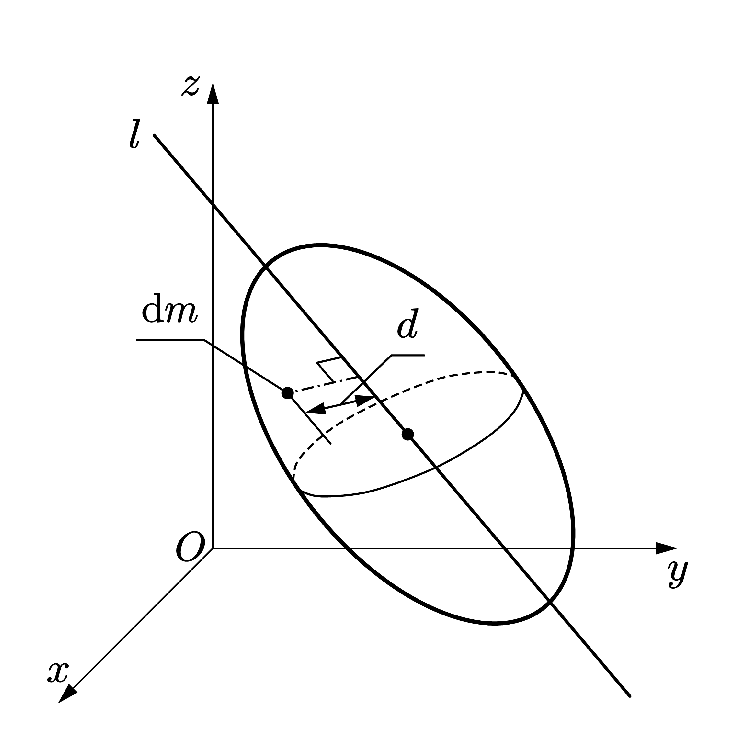
\includegraphics[width=5cm]{inertia.pdf}
    \caption{转动惯量示意}
\end{wrapfigure}

\paragraph{与力学专业内容的联系}
微积分将伴随我们后续整个学习生涯,几乎没有哪一个力学专业课用不到微积分,我们只介绍几个典型应用。
\begin{itemize}
    \item 质心与转动惯量——重积分
          \[
              \symbfit{r}_C=\dfrac{\int_\Omega \symbfit{r}\,\mathrm{d}m}{\int_\Omega \mathrm{d}m}, \quad J_l=\int_\Omega d^2\,\mathrm{d}m
              .\]
    \item 建立连续体平衡微分方程——微元法
          \[
              \tau_{xy} = \tau_{yx}\quad \text{\itshapeCJK(切应力互等)}
              .\]
    \item     弹性力学中轴对称问题应力函数所满足的方程
          \[
              \left( \frac{\mathrm{d}^2}{\mathrm{d}\rho ^2}+\frac{1}{\rho}\frac{\mathrm{d}}{\mathrm{d}\rho} \right) ^2\varPhi =\frac{\mathrm{d}^4\varPhi}{\mathrm{d}\rho ^4}+\frac{2}{\rho}\frac{\mathrm{d}^3\varPhi}{\mathrm{d}\rho ^3}-\frac{1}{\rho ^2}\frac{\mathrm{d}^2\varPhi}{\mathrm{d}\rho ^2}+\frac{1}{\rho ^3}\frac{\mathrm{d}\varPhi}{\mathrm{d}\rho}=0
              .\]
          ——Euler方程

    \item  信号频谱分析——Fourier级数,见 \autoref{fig:一种信号的时域与频域关系对应图}
\end{itemize}



\begin{figure}
    \centering
    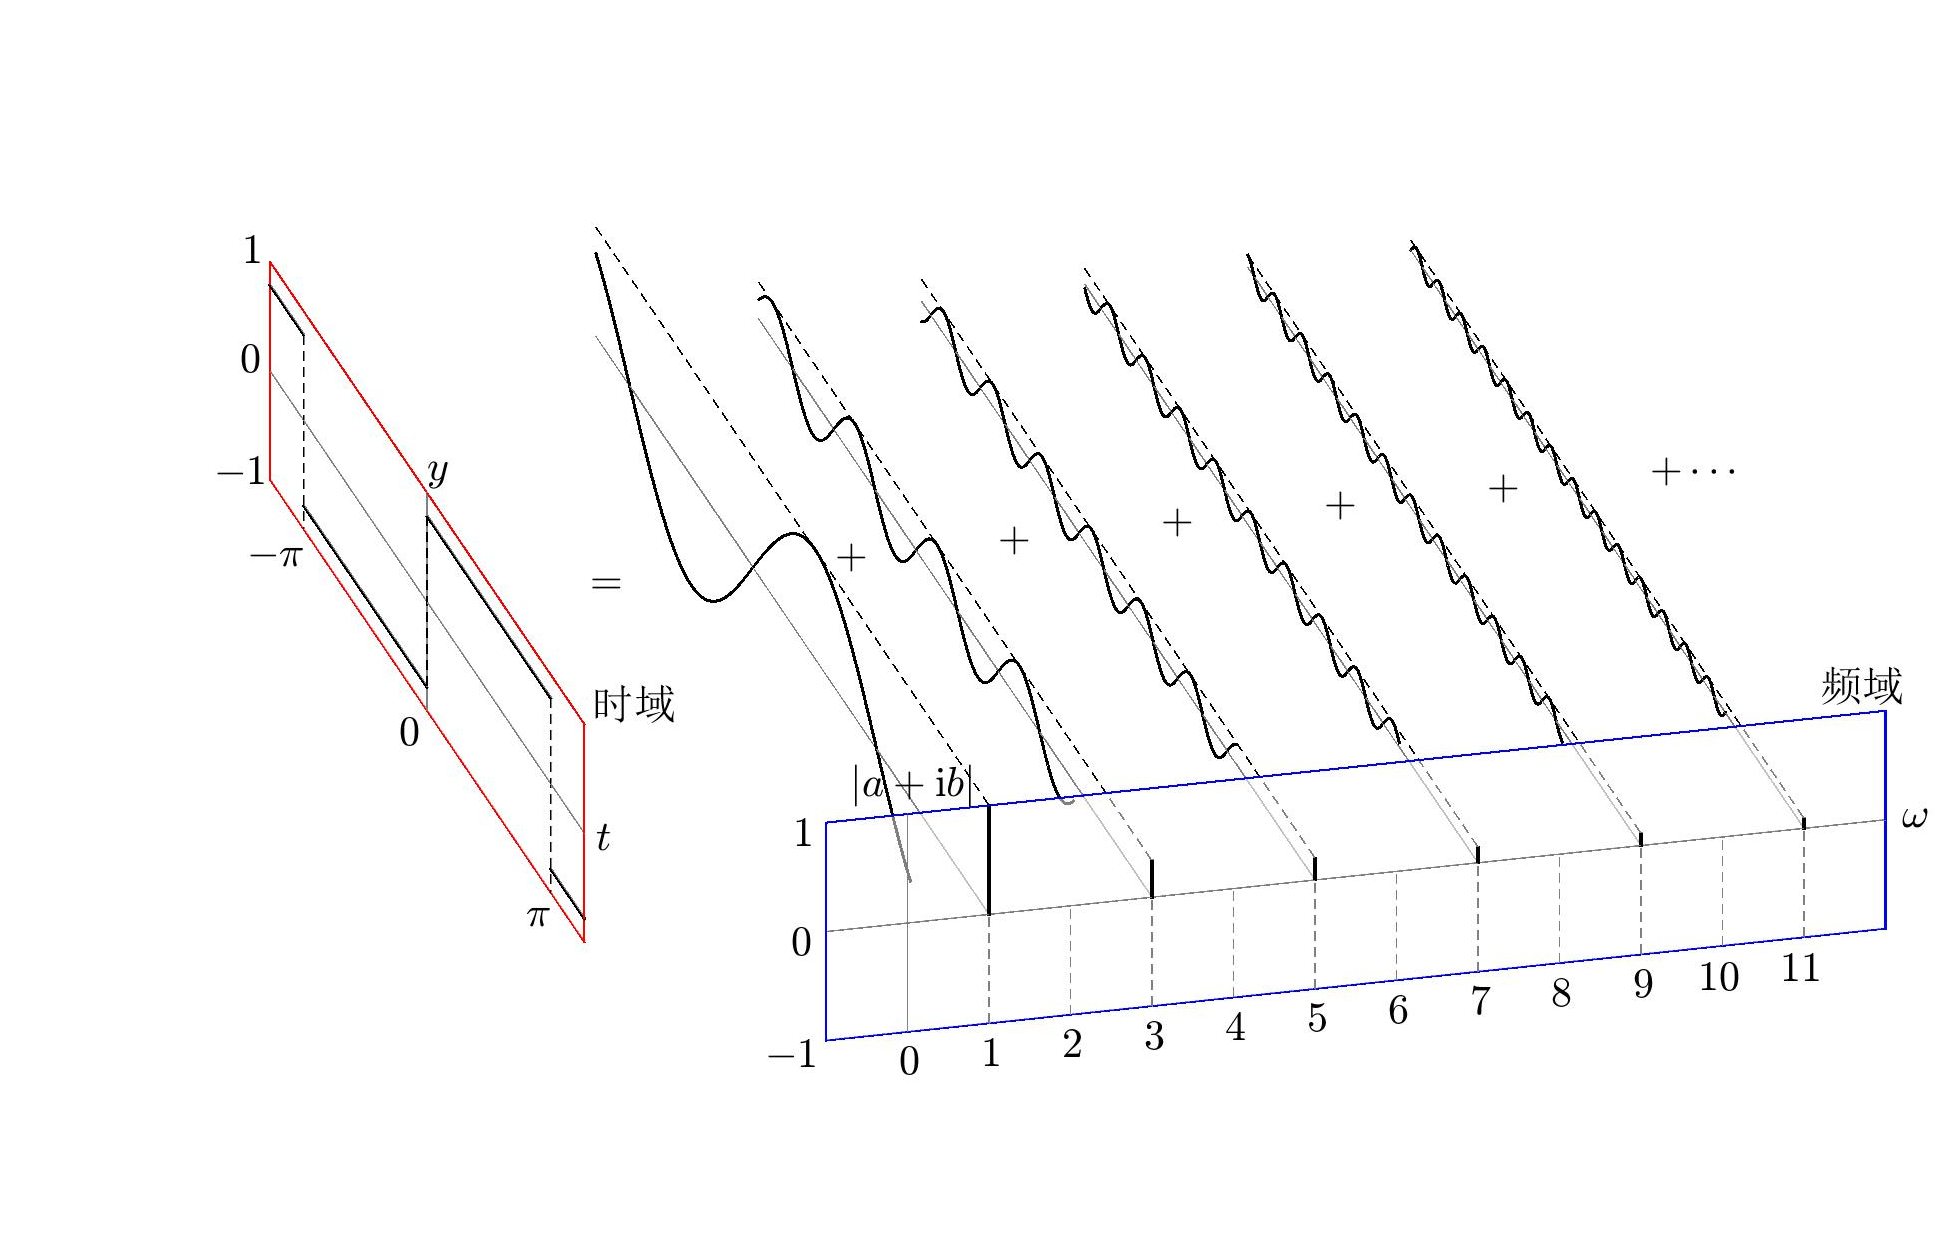
\includegraphics[scale=0.45]{Fourier_series.pdf}
    \caption{一种信号的时域与频域关系对应图}
    \label{fig:一种信号的时域与频域关系对应图}
\end{figure}

\paragraph{学习建议}

我们以后的运用以计算为主,如果初学时对一些严格定义有困惑,可以在不影响计算与运用的前提下适当放一放。在能进行计算的前提下,回头结合计算实例进行理解。

以计算为主不代表要去算各种奇奇怪怪的极限、积分。如果没有准备竞赛的要求或是出于个人兴趣爱好,没有必要算那些奇怪的积分(特别是有些来路不明的钓鱼题)。一来,能够计算出结果的积分是十分有限的,更可能要用到许多特殊函数的性质;二来,我们以后会用数值方法去处理广泛的积分,若非分析性质的需要,数值解是足够的。

一般微积分课程中对于矢量分析的内容是不足的,这里可以做一些额外补充,否则面对普通物理学当中的力学推导,以及理论力学当中的运动学部分的推导可能会比较吃力,推荐书目有 \textcite[托马斯大学微积分]{李伯民2009托马斯大学微积分} 的10、11两章,\textcite[数学分析新讲]{张筑生数学分析},\textcite[工程数学——矢量分析与场论]{谢树艺2015工程数学} 的前2章。

\paragraph{参考书目}

参考书选择大前提:一定要适合自己,不要三人成虎,先入为主地迷信或厌恶某本教材!学习过程中可广泛参考不同教材,但应该以其中一两本为主,其余为辅。

首先,同济大学的《高等数学》能够满足正常的微积分知识学习,包括很多高中参加物理竞赛的同学学习高数时也参考了这本书。这本书的例子、逻辑与习题量至少能满足力学专业的学习,如果要参考其他教材,请至少以此为下限进行参考。这套教材最大的问题是过于中庸,虽然有例子但不够丰富,逻辑性与严密性卡在一个比较尴尬的位置。

\begin{itemize}
    \item 入门级参考书:

          \begin{center}
              
\includegraphics[scale=0.6]{book/1.png} \quad
              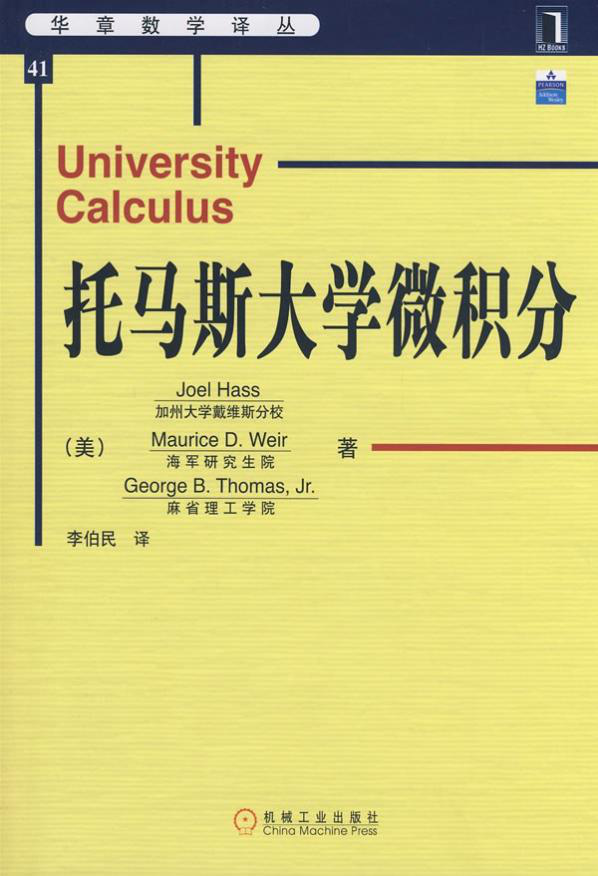
\includegraphics[scale=0.6]{book/2.png} \quad
          \end{center}

          \begin{itemize}
              \item \textcite[普林斯顿微积分读本]{杨爽2010普林斯顿微积分读本}

                    入门级微积分读本,适合没有相应数学基础的高中生以及文、史、哲、法学生阅读,主体内容是一元微积分的部分。这本书的特点是起点足够低,对于基础内容的讲解也足够细致,不一味强调严谨性,因而适合初学者入门。问题在于内容较浅、过于冗杂,这种风格并不适合一般理工科的后续学习和科研要求。

              \item \textcite[托马斯大学微积分]{李伯民2009托马斯大学微积分}

                    入门级微积分读本,基本涵盖了国内一般微积分教材的大部分内容。特点是起点低,知识点引入比较流畅,内容丰富,实例、图示与习题都很充足,也很适合初学者入门。
                    后续的数学课程帮助很大。
          \end{itemize}

    \item 进阶与拓展参考书:
          \begin{center}
              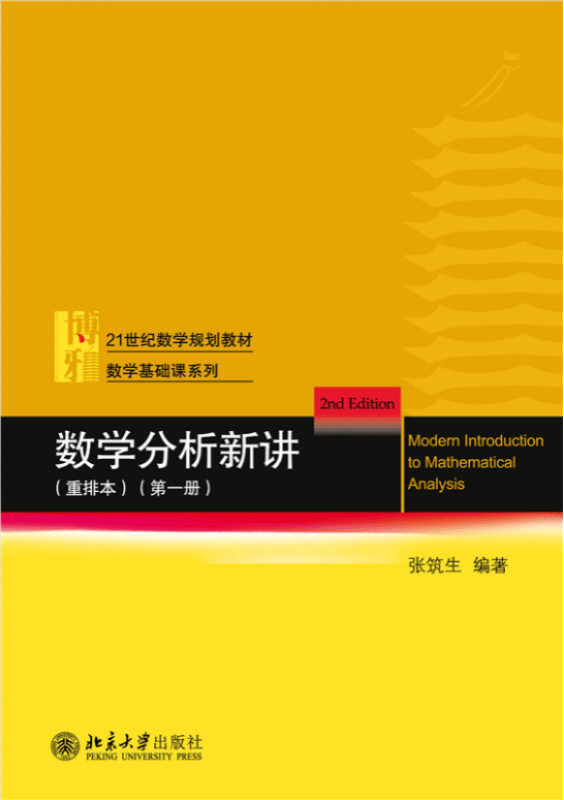
\includegraphics[scale=0.35]{book/5.png} \quad
              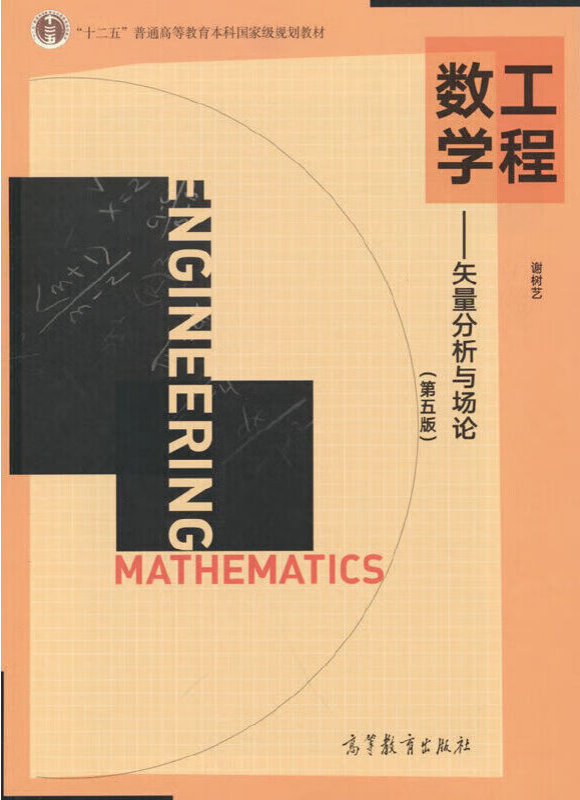
\includegraphics[scale=0.35]{book/3.png} \quad
              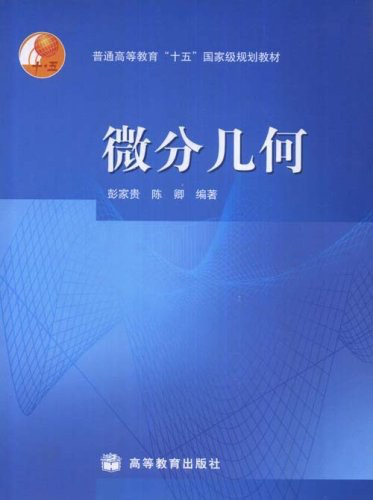
\includegraphics[scale=0.56]{book/4.png}
          \end{center}
          \begin{itemize}
              \item \textcite[数学分析新讲]{张筑生数学分析}

                    这一套书作为数学分析来说,没有在集合论和实数上大书特书,更多地是从计算以及几何意义的角度进行引入。对于书中提及的拓扑和一般线性空间的内容,只需要粗略扫过,有一个印象即可。书中对于多元微积分的处理,曲面以及曲线积分的计算,矢量微分算子的引入都是非常有借鉴价值的,尤其是微分方程部分,包括常微分方程和简单的偏微分方程理论,对学习后续的数学课程帮助很大。

              \item \textcite[工程数学——矢量分析与场论]{谢树艺2015工程数学}

                    这本书在微积分水平上对矢量分析进行了比较全面的讨论,第一章讨论了矢量函数的微积分,后边讨论了矢量场、梯度算子及一般的曲线坐标系中的运算,对于本科课程级别的运动学、弹性力学和流体力学中的矢量运算比较有帮助。

              \item \textcite[微分几何]{彭家贵2002微分几何}

                    这本书所讲的第一部分是古典微分几何的内容,适合在学了微积分之后适当阅读。涉及的数学工具只有微积分、空间解析几何及少量的线性代数,理论不抽象,计算较复杂,同时,工程力学的研究大都是在经典的三维欧氏空间$\mathbb{R}^3$下的,所以这本书正适合力学专业的同学阅读。

                    古典微分几何大致可分为曲线论和曲面论。曲线论的研究方法可以追溯到对质点运动轨迹的研究,比较有意思的是标架方法,学过这一部分内容之后正好可以重新审视一下质点运动学的内容。曲面论的内容相对比较丰富,一般来说会先从曲面的基本形式和曲率入手,通过活动标架方法,研究曲面的结构方程,最后是曲面的内蕴几何学及测地线的理论。
          \end{itemize}
\end{itemize}


\subsubsection{线性代数}

\paragraph{主体知识介绍}

线性代数以研究\uwave{线性变换}、\uwave{线性方程组}为主。在数学上,\textbf{线性}一般指的是\uwave{齐次性}和\uwave{可加性},例如对于映射$f:\mathbb{R}^n\to\mathbb{R}$,这两条性质指的是

\begin{itemize}
    \item 齐次性:$f(a\symbfit{x})=a\cdot f(\symbfit{x})$.

    \item 可加性:$f(\symbfit{x}+\symbfit{y})=f(\symbfit{x})+ f(\symbfit{y})$.
\end{itemize}
这时就说映射$f$是线性的。研究在有限维线性空间(例如$n$维欧氏空间$\mathbb{R}^n$)中线性变换的代数性质的分支就是线性代数。那么典型的线性变换有哪些呢?我们举平面解析几何中的两个例子说明。

设平面上有一点$(x,y)$,现在将其绕原点逆时针旋转$\theta$度,利用三角函数的诱导公式容易得到变换后点$(x',y')$的坐标为
\[
    \begin{cases}
        x'=x\cos \theta -y\sin \theta, \\
        y'=x\sin \theta +y\cos \theta.
    \end{cases}
\]
不妨将点$(x,y)$看作是矢量$(x,y)$。在这里看来,齐次性就是在变换先后将向量$(x,y)$拉长若干倍;可加性可看成将向量$(x,y)$拆成$(x,0)$与$(0,y)$之和,将二者分别逆时针旋转$\theta$度后再加和,得到的结果与直接旋转向量$(x,y)$是一致的。所以,这种旋转变换是线性变换。

\begin{figure}[h]
    \centering
    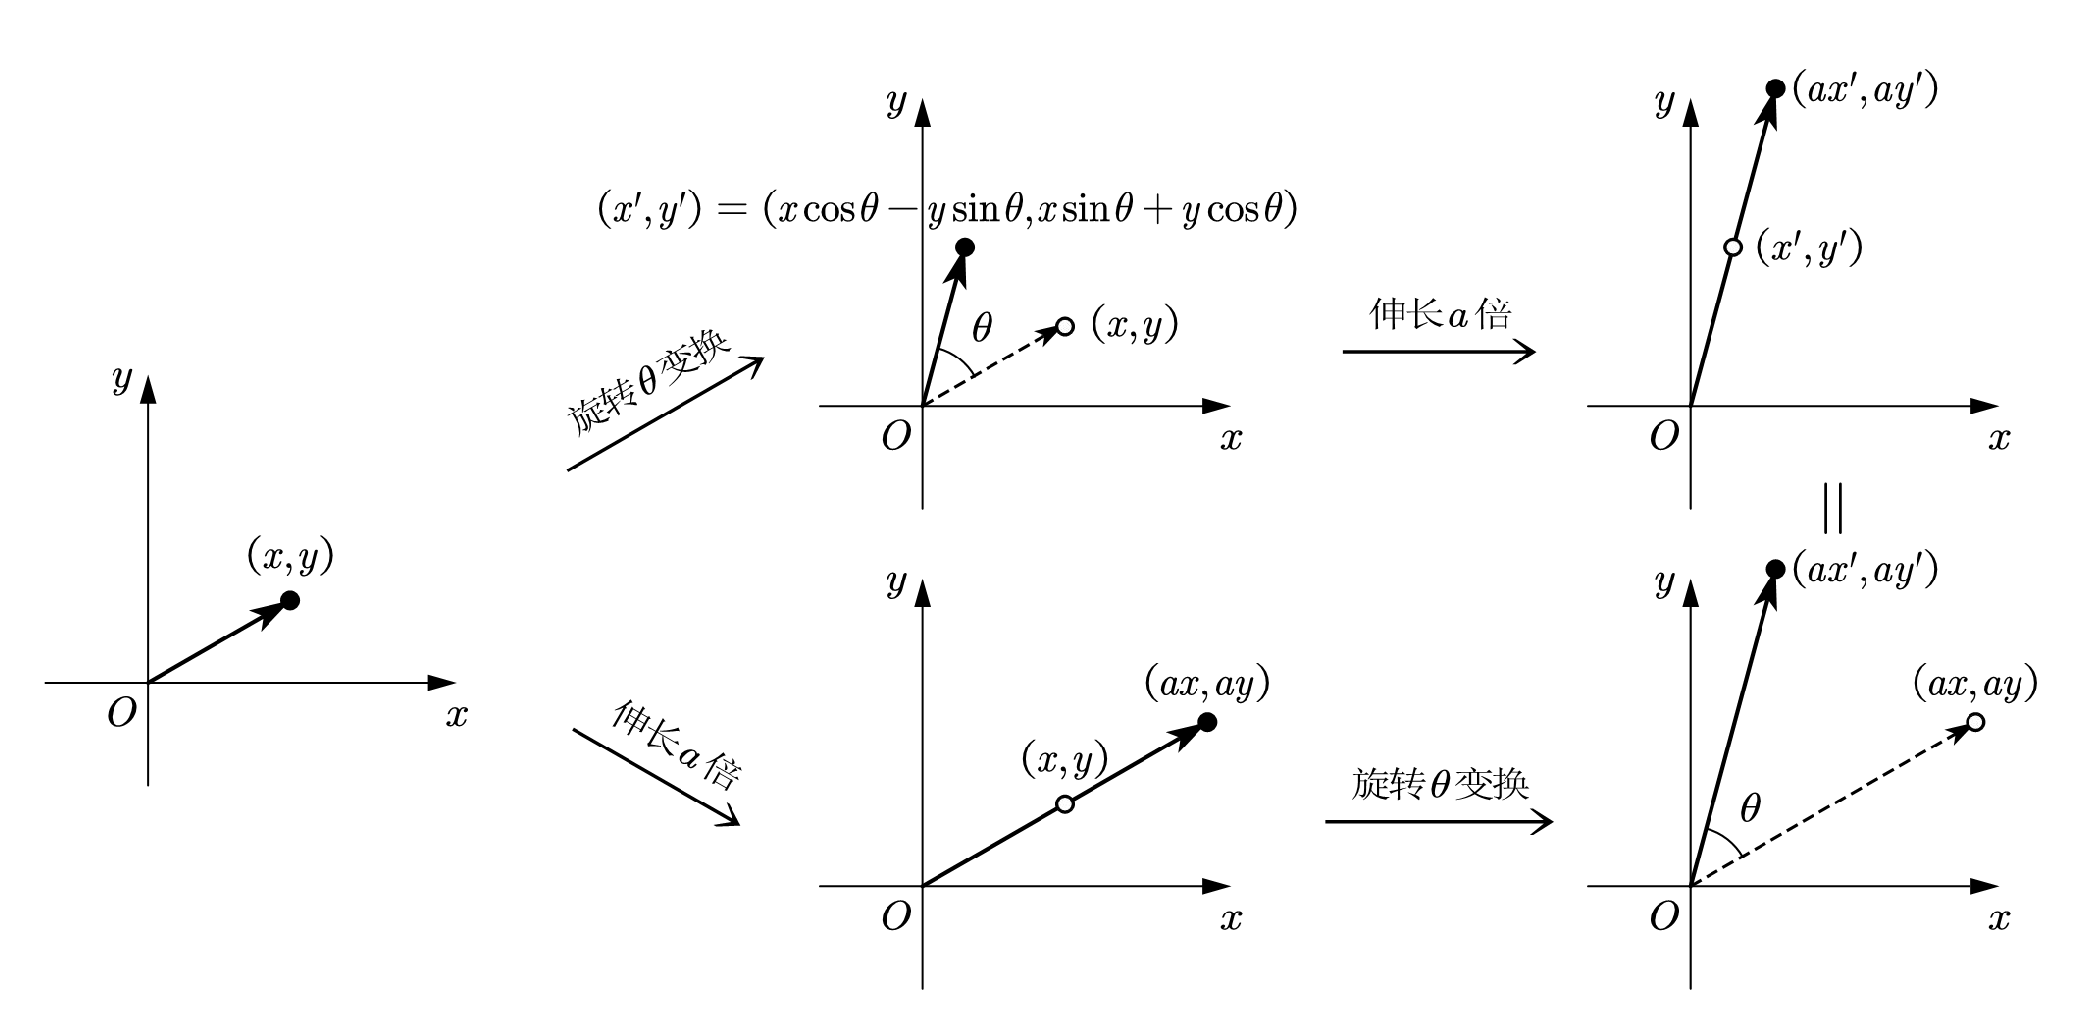
\includegraphics[width = 0.8\linewidth]{homogeneity.pdf}
    \caption{验证旋转变换的齐次性}
\end{figure}


\begin{figure}[h]
    \centering
    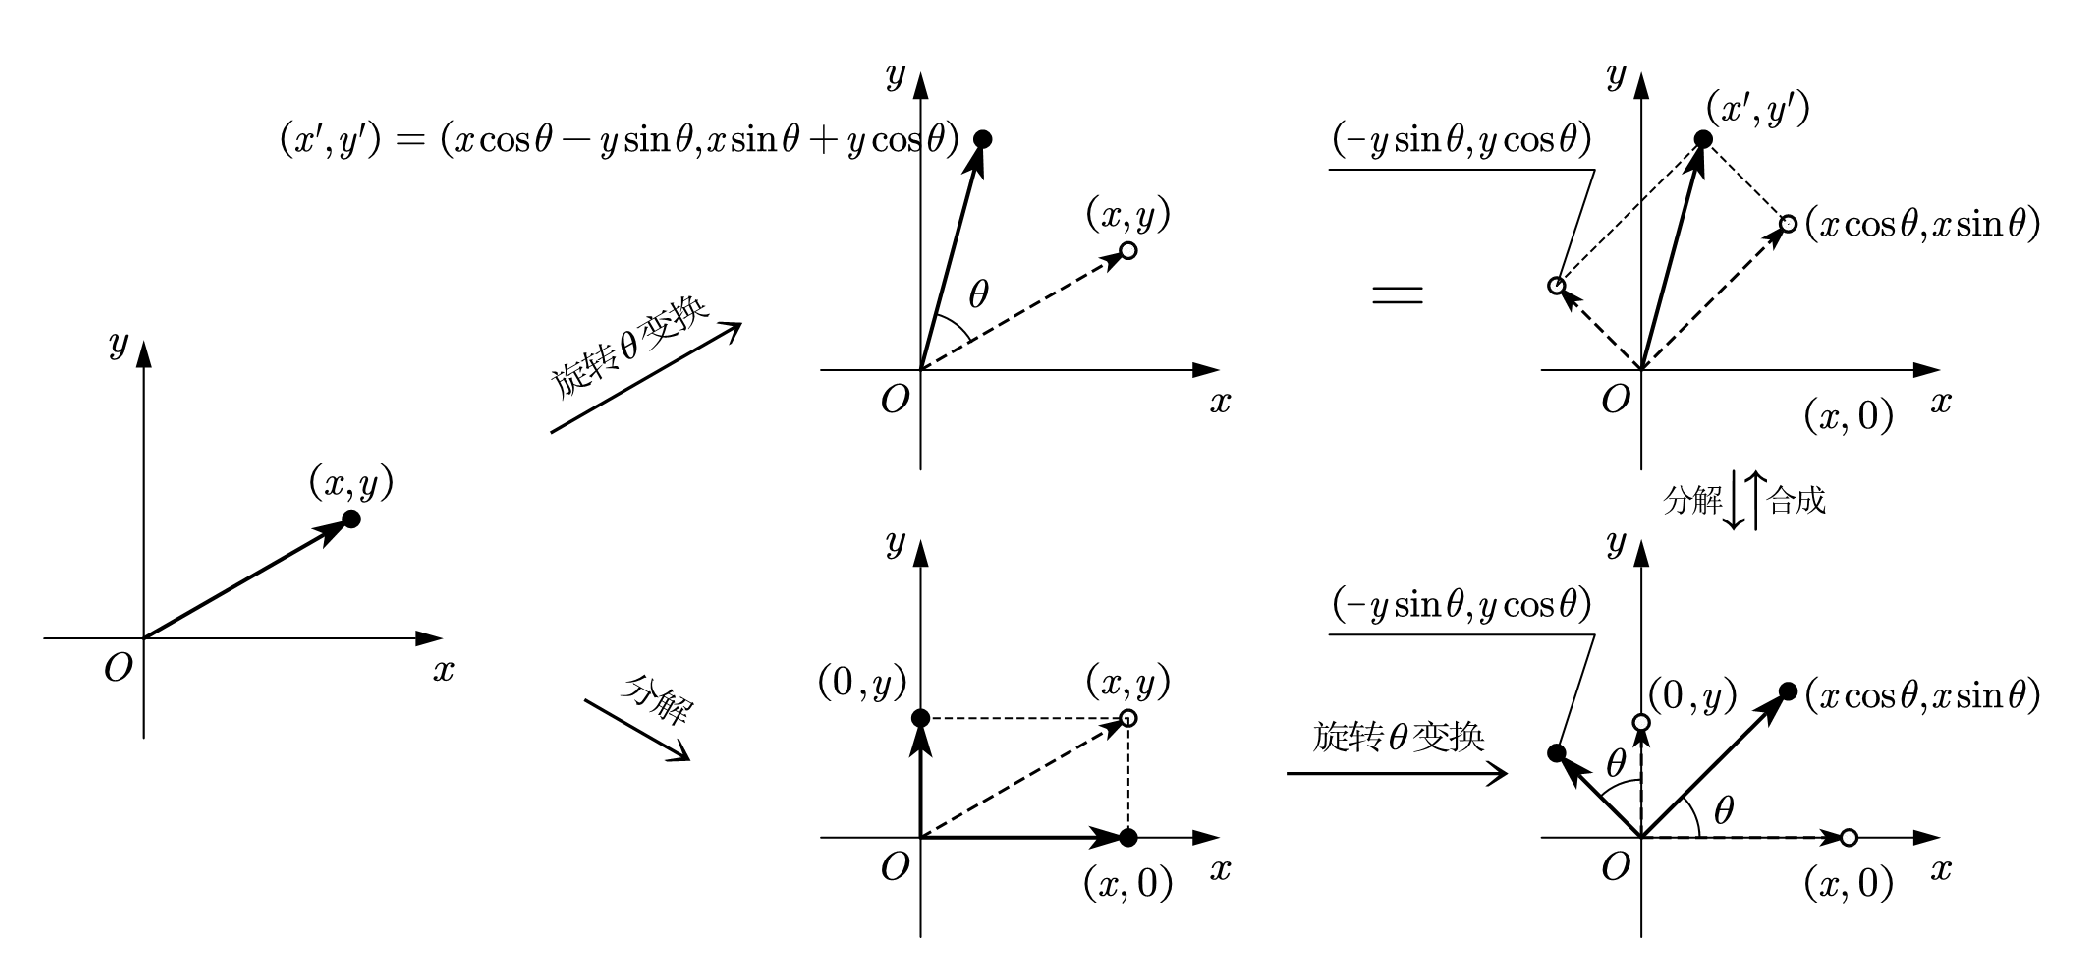
\includegraphics[width = 0.8\linewidth]{additivity.pdf}
    \caption{验证旋转变换的可加性}
\end{figure}


下面来考察将点$(x,y)$平移$(a,b)$之后的结果,即
\[
    \begin{cases}
        x'=x+a, \\
        y'=y+b. \\
    \end{cases}
    \]






% \begin{center}
%     % 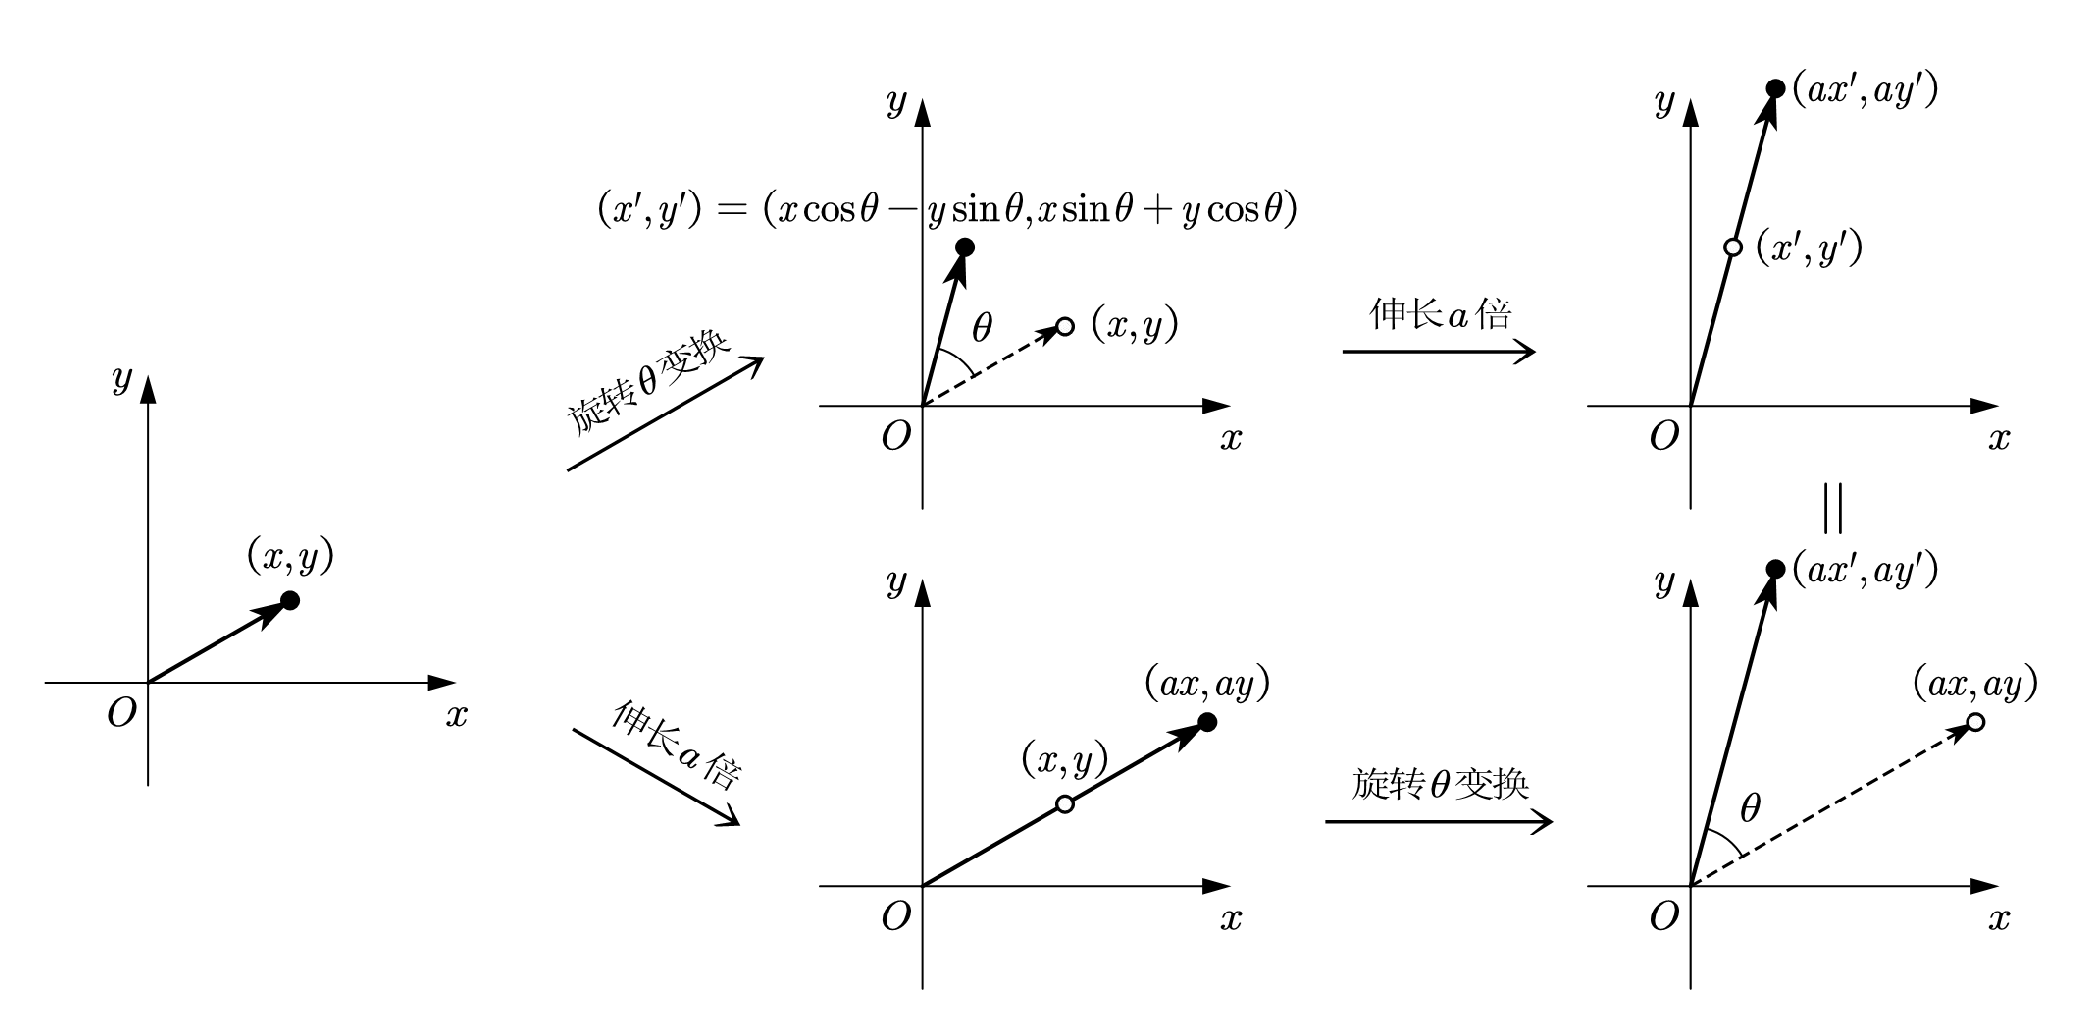
\includegraphics[scale=0.45]{homogeneity.pdf}
%     \addtocounter{figure}{1}
%     \small 图\thesubsection.\thefigure 验证旋转变换的齐次性 \normalsize
% \end{center}
% \begin{center}
%     % 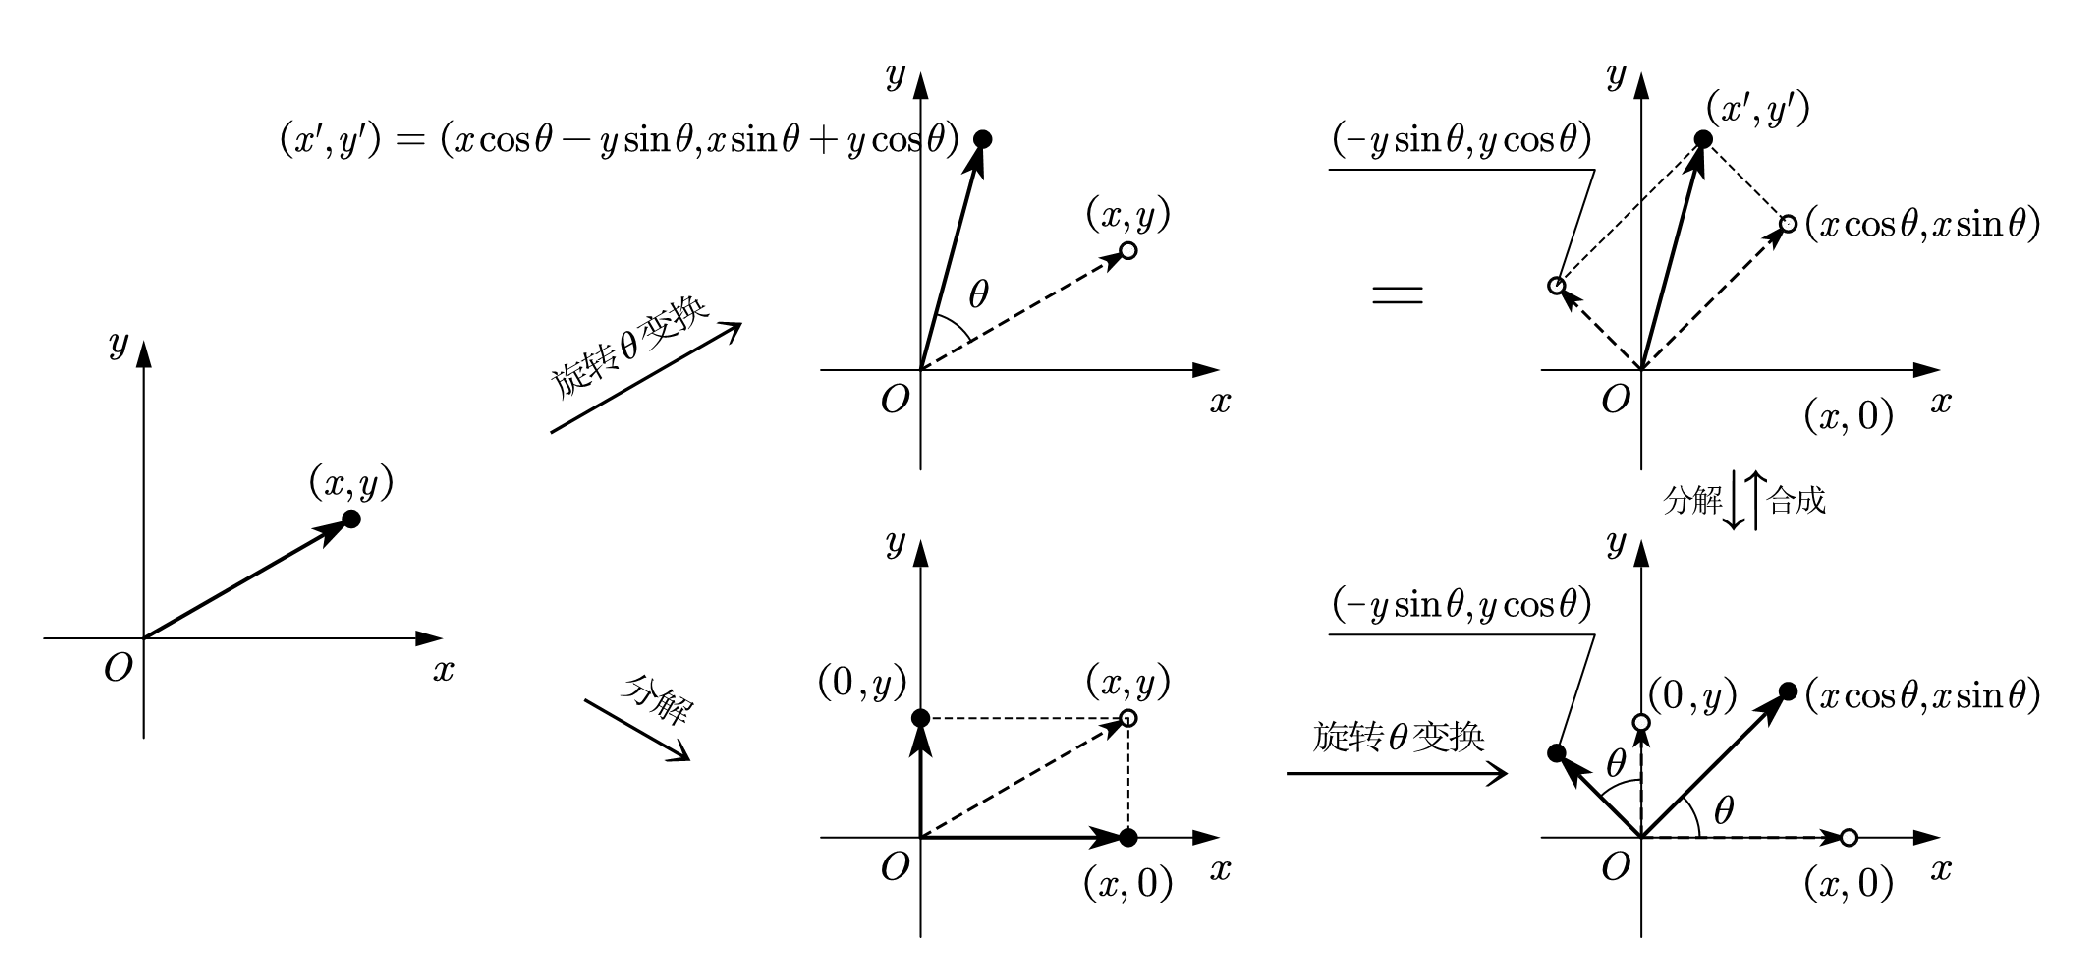
\includegraphics[scale=0.45]{additivity.pdf}
%     \addtocounter{figure}{1}
%     \small 图\thesubsection.\thefigure 验证旋转变换的可加性 \normalsize
% \end{center}

我们说这个变换不满足齐次性,也不满足可加性。仅以齐次性为例说明,将平移变换记为$f$,则$f(x,y)=(x+a,y+b)$,对于任意一个给定的$k$,$f(kx,ky)=(kx+a,ky+b)\ne (kx+ka,ky+kb)$。从几何直观上来看,先将向量$(x,y)$伸长$k$倍,再将箭头的位置平移$(a,b)$,与先将向量$(x,y)$箭头的位置平移$(a,b)$,再将其伸长$k$倍的结果显然是不一样的。类似也能验证可加性不成立。但是,如果我们将点$(x,y)$视为三维空间中的向量$(x,y,z)$,并规定新的平移变换为

\begin{align*}
    \begin{cases}
        x'=x+az, \\
        y'=y+bz, \\
        z'=z .   \\
    \end{cases}
\end{align*}

能够验证,这样规定的平移变换又是满足齐次性和可加性的了,因而是线性变换。同时,$z$的选取是任意的,为了与平移的单位一致,直接令$z=1$。

\begin{figure}[h]
    \centering
    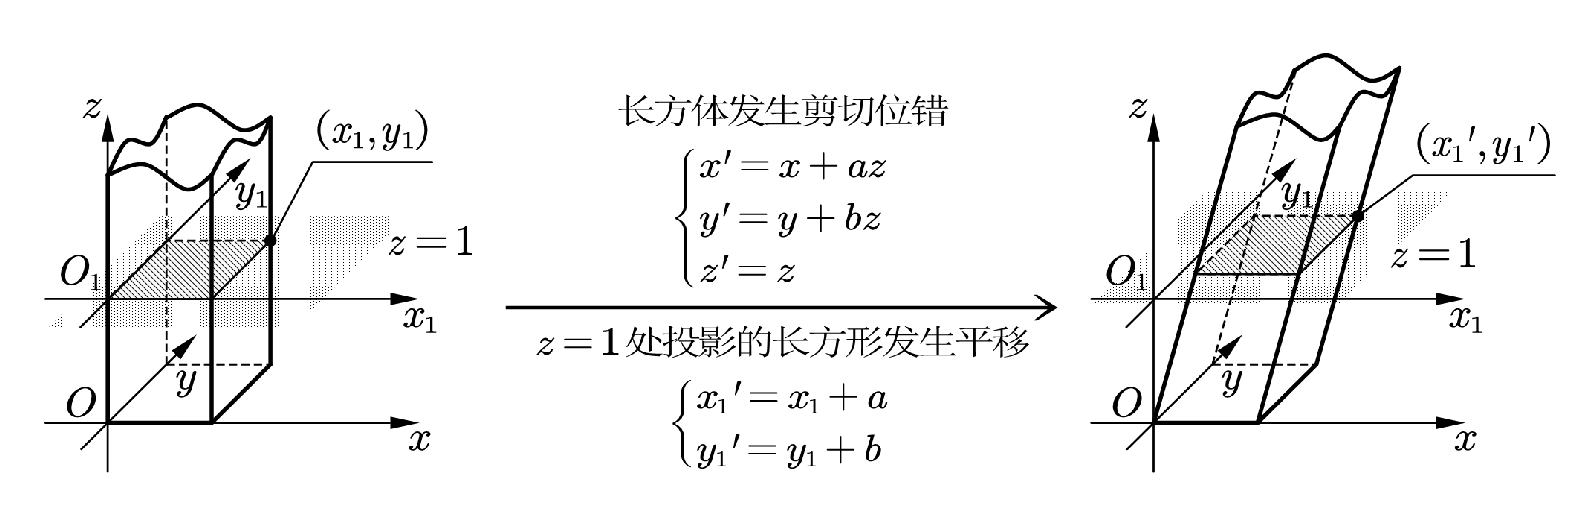
\includegraphics[scale=0.5]{shear.pdf}
    \caption{新规定的平移变换,用三维空间中的线性变换描述二维空间中的平移}
\end{figure}

借由上边两个线性变换,我们还能够发现,如果已知线性变换的规则以及变换后的结果,返回去求变换前的点的过程,实际上就是解线性方程组。因此,解线性方程组也与线性变换紧密关联。

在这个阶段,我们通常只研究实数域内的线性变换。线性变换都能写成\textbf{矩阵},矩阵是一张二维数表,我们再规定矩阵的基本运算规则,使得线性变换作用在向量上能够写成线性变换与向量相乘,就能对线性变换进行研究了。矩阵除了加减、数乘,还有许多其他运算,如\uwave{矩阵相乘}、\uwave{行列式}、\uwave{逆}、\uwave{转置}、\uwave{秩}等等,这些运算是帮助我们研究线性变换的有力工具。

线性变换的作用对象是\uwave{向量},所以我们也要研究向量、向量组和向量空间。向量组\uwave{线性相关/线性无关}的概念很常用,后续学习中它将反复出现。向量空间中最重要的概念是\uwave{基向量},所以我们会研究如何在一个向量空间中“选出”一组比较好的基向量(\uwave{Schmidt正交化})。特别的,我们会研究欧氏空间$\mathbb{R}^n$,它比一般的线性空间多了\uwave{内积}和\uwave{距离}这两个概念,而三维欧氏空间$\mathbb{R}^3$,也就是我们熟知的现实中的三维空间,其上又有\uwave{叉乘}这一运算,这些是研究空间解析几何的基本工具。

解线性方程组是线性代数中很重要的一部分,不过事实上我们并不常用Cramer法则,更多的是用\uwave{Gauss消元法}(\uwave{初等变换法})。通过计算低阶的线性方程组要掌握这套流程,至于高阶的线性方程组可以尝试编程实现,在后续的课程中也会讨论解更大规模线性方程组的数值方法。

研究同一线性变换连续作用于向量若干次产生了对\uwave{特征值}与\uwave{特征向量}相关内容的研究。一些方阵(行、列元素个数相等的矩阵)能够写成$\symbfit{P}^{-1}\symbfit\Lambda \symbfit{P}$,其中$\symbfit{\Lambda}$是对角矩阵(主对角线以外的元素都是$0$的矩阵),称这个过程为矩阵的\uwave{相似对角化}。根据矩阵乘法的结合律,问题转化为对角矩阵的幂的计算,而这是容易的。特征值与特征向量不仅能用于求矩阵的幂,还能用来求微分方程和差分方程,相似关系还可以描述同一个线性变换在不同基下的表示。此外,有一些矩阵具有特定的性质,如\uwave{正交矩阵}、\uwave{对称矩阵}等需要注意。例如,正交矩阵的一个良好的性质是它表示等距变换。

线性代数课程中一般还会介绍\uwave{二次型}理论。二次多项式也可以用矩阵表示,而二次多项式与空间曲面密切相关,所以这部分内容可以与空间解析几何相联系。


除了以上这些基本知识,还可以做适当的补充,包括多项式、Jordan标准型以及线性空间。

\paragraph{与力学专业内容的联系}

\begin{itemize}
    \item 应力、应变极值方向分析——特征值与特征向量问题

    \item 结构力学中的力法方程、有限元方程——求解线性方程组

    \item 多自由度系统模态分析——广义特征值与特征向量问题
\end{itemize}

\paragraph{学习建议}

在学习线性代数时,一个比较好的做法是寻找实例和做推广。例如,定积分运算满足Cauchy-Schwarz不等式
\[
    \left|\int_{a}^{b}f(x)g(x)\,\mathrm{d}x\right|\leqslant\left|\int_{a}^{b}(f(x))^2\mathrm{d}x\right|\cdot \left|\int_{a}^{b}(g(x))^2\mathrm{d}x\right|
    .\]
而在欧氏空间部分,我们也有一个基于内积定义推导出的Cauchy-Schwarz不等式
\[
    \left|\langle a,b\rangle\right|\leqslant\left|\langle a,a\rangle\right| \cdot \left|\langle b,b\rangle\right|
    .\]
由此可以想到,积分运算是不是某种意义上的内积呢?这种类比、抽象的思考方式在代数的学习中是比较重要的,不必拘泥于课本上的内容,最好要广泛联系,多多思考。无论如何,偏向代数的数学第一位是理解概念、寻找动机,然后才可能是在此基础上做各种计算。

一般的线性代数课程所讲内容未免略显单薄。为此,最好补充关于Jordan标准型、线性空间的知识,以及线性代数的一些具体应用,推荐书目有\textcite[普通高中课程标准实验教科书\ 数学\ 选修4-2\ A版\ 矩阵与变换]{矩阵与变换}、\textcite[线性代数高级教程——矩阵理论及应用]{线性代数高级教程}、\textcite[线性代数应该这样学]{阿克斯勒杜现昆2016线性代数应该这样学}。

\paragraph{参考书目}

目前绝大多数国内的线性代数教材都采用开篇讲行列式的模式,稍好一些的教材会直接跟进解线性方程组的Cramer法则。线性代数的基本理论比较琐碎,也是本科期间接触到的第一门思维模式与以往不同的数学课,然而行列式起手的这种讲法并不够合理,线性代数最核心、最重要的内容应当是线性变换,次之为解线性方程组,直接引入行列式很容易让初学者不知所云。所以,这里推荐三本引入较为自然的教材,目的是提纲挈领,先对线性代数形成一个大致印象,知道线性代数在研究什么。

\begin{itemize}
    \item 入门级参考书:
          \begin{center}
              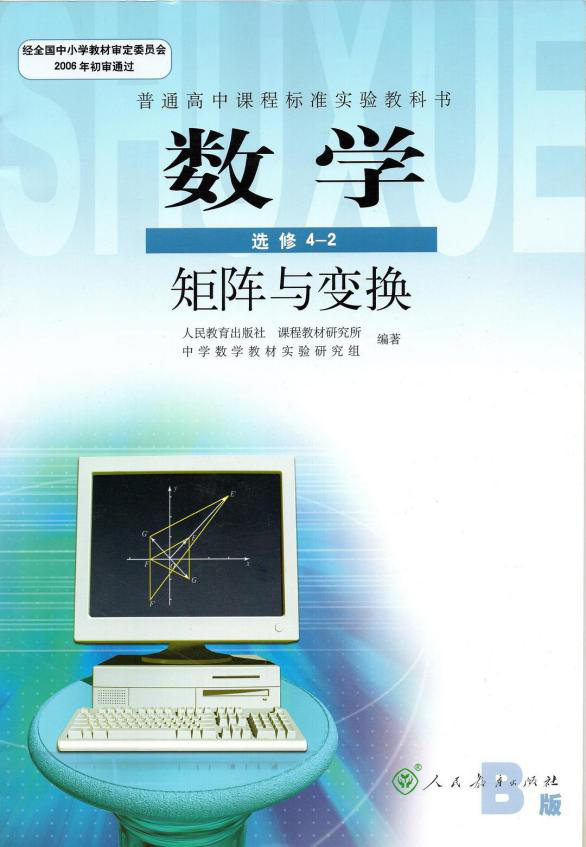
\includegraphics[scale=0.6]{book/6.png} \quad
              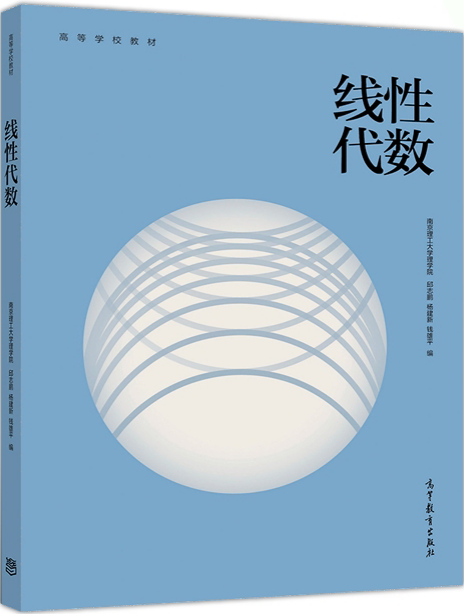
\includegraphics[scale=0.46]{book/7.png} \quad
              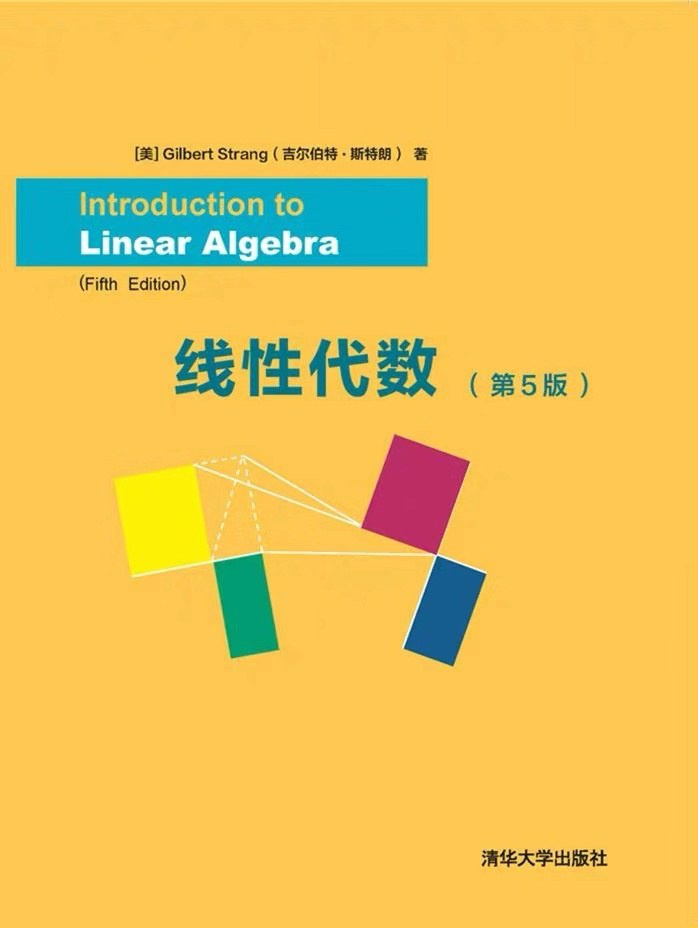
\includegraphics[scale=0.3]{book/8.png}
          \end{center}

          \begin{itemize}
              \item \textcite[普通高中课程标准实验教科书\ 数学\ 选修4-2\ A版\ 矩阵与变换]{矩阵与变换}

                    这本书是旧版高中教材,并且目前已经不将这本书的内容作为高考内容,但这本教材通过平面解析几何引入线性变换和矩阵的做法是很好的,用线性变换将整个线性代数串了起来,思路十分清晰。不足之处是主要只讨论了二阶矩阵的理论,所以不太适合完整的线性代数的学习。

              \item \textcite[线性代数]{线性代数}

                    这本教材是少有的从线性变换讲起的国内教材,引入矩阵也比较自然。并且还有一个亮点是这本书在附录部分给出了平面解析几何中线性变换的几何含义。尽管在引入部分做得很好,但总的知识量与国内其他教材并无差异。

              \item \textcite[线性代数:第5版]{线性代数5}

                    并不是说从解线性方程组起讲的教材都不好,这本教材就是从线性组合和解线性方程组引入的,引入也很自然、直观。同时,这本书中包含了奇异值分解、复矩阵以及其他线性代数的应用,如快速Fourier变换、最小二乘近似、图像处理等内容,就实用性这一点来说是很棒的。
          \end{itemize}

    \item 进阶与拓展参考书:

          线性代数的进阶便是矩阵理论,所以,其他的推荐书目我们都放在矩阵理论部分。
\end{itemize}





\subsection{进阶数学培养}

在学习过微积分和线性代数后,一些学校会选择在本科阶段开设进一步的数学课程,以满足专业学习的需要,这里介绍最基本的几门数学课程。

\subsubsection{概率论与数理统计}

\paragraph{前置知识:}微积分

\paragraph{部分知识介绍}

条件概率的Bayes公式,建立先验概率与后验概率的联系。

常用的随机变量分布及其数字特征。常用的离散分布有二项分布、Poisson分布、几何分布,连续分布有均匀分布、指数分布、正态分布、Weibull分布。数字特征则是期望、方差和协方差。

数理统计当中的几个分布和参数估计。重要的分布有$\chi^2$分布、$t$分布、$F$分布。参数估计主要是矩估计和最大似然估计。

\paragraph{与力学专业内容的联系}

\begin{itemize}
    \item 零件可靠性/寿命分析——Weibull分布及特征量

    \item 随机振动——随机过程的统计特征
\end{itemize}

\paragraph{学习建议}

对于大部分做力学相关的同学来说,用到概率论与数理统计的情形其实不多,能应付考研即可。笔者也很难给出合适的建议,最好还是要熟悉基本的运算、了解一些常用的概率分布、其应用场合以及基本的统计方法,这可能在大规模的数据处理方面派上用场。另一方面,尽管有关于湍流的统计理论研究,但目前从事这方面研究的比较少,而且这里所学的概率论和统计学的基础知识大概是不够用的,不展开介绍了。


\subsubsection{复变函数与积分变换}

\paragraph{前置知识:}微积分

\begin{wrapfigure}{r}{6cm}
    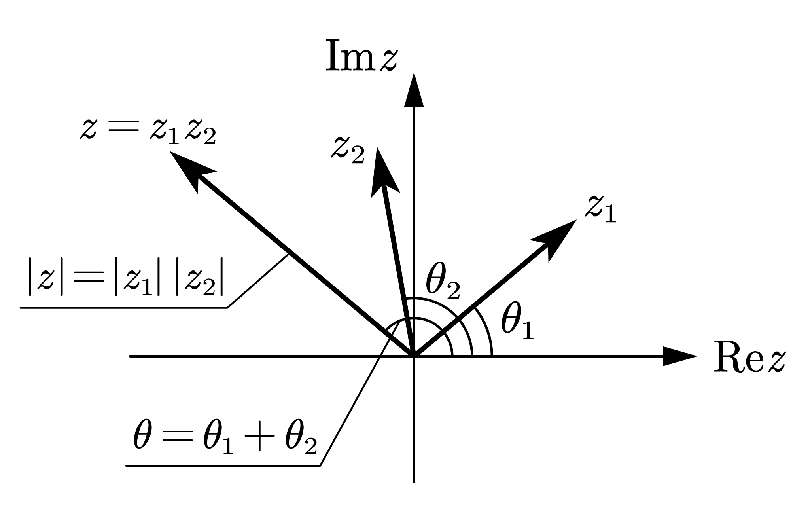
\includegraphics[scale=0.45]{mult_z.pdf}
    \caption{复数乘法的运算法则}
\end{wrapfigure}

\paragraph{部分知识介绍}

复变函数指的是函数的定义域和值域都是复数的函数,这门课上只研究自变量是一个复数的情形。一个复数$z\in\mathbb{C}$可以写成$z=x+\mathrm{i}y, x,y\in\mathbb{R}$的形式,也就是说复变函数与二元实函数很像,可以把这门课当作是二元微积分的升级版。但复数毕竟不同于一般的二维向量,在复变函数这门课里会有更多的结论。

首先要熟悉复数的基本运算,复数与二维欧氏空间中的向量十分相似,不仅可以用平面表示,向量可以进行的所有运算复数也可以进行。但复平面$\mathbb{C}$与二维平面$\mathbb{R}^2$最重要的区别是复数上有“真正的”乘法,注意一般的$\mathbb{R}^2$上只定义了数乘
\[
    f:\mathbb{R} \times \mathbb{R}^2  \to \mathbb{R}^2,~ (a,\symbfit{x})  \mapsto a\symbfit{x}
    .\]
和内积

\[
    f:\mathbb{R}^2 \times \mathbb{R}^2\to \mathbb{R},~(\symbfit{x}_1,\symbfit{x}_2) \mapsto a
    .\]



因为这种映射的“乘数”和“结果”形式不统一,所以说它们不是“真正的”乘法,而不曾定义
\[
    f:\mathbb{R}^2 \times \mathbb{R}^2\to \mathbb{R}^2,~(\symbfit{x}_1,\symbfit{x}_2) \mapsto \symbfit{y}
    .\]
这样的“真正的”乘法。在复平面上则有满足$\mathbb{C} \times \mathbb{C} \to \mathbb{C}$的乘法,这是因为复数比一般的二维平面多了$\mathrm{i}^2=-1$这样一个定义。这导致复变函数的推论远比一般的二元实函数要多。

认识了基本的复变函数后,首先要讨论的就是可导/可微的概念,这里我们最关注的是一类被称为\uwave{解析函数}的复变函数。一般的复变函数$f$是可以看成两个关于$x,y$的实函数的,而注意$z,\bar{z}$(即$z$的共轭)是线性无关的,所以一般的复变函数可以看成是关于$z,\bar{z}$的二元函数。解析这个性质说的其实就是在定义域上,$f$对$z$可导,同时与$\bar{z}$无关,后者就是Cauchy-Riemann条件:
\begin{align*}
    \frac{\partial f}{\partial \bar{z}}=0 \Longleftrightarrow
    \begin{dcases}
        \dfrac{\partial u}{\partial x}=\dfrac{\partial v}{\partial y},  \\
        \dfrac{\partial v}{\partial x}=-\dfrac{\partial u}{\partial y}. \\
    \end{dcases}
\end{align*}
解析函数的性质很好:无穷次可微、实部与虚部分别满足\uwave{调和方程},即设$f(z)=u(x,y)+\mathrm{i}v(x,y)$,则
\begin{align*}
    \begin{dcases}
        \dfrac{\partial ^2u}{\partial x^2}+\dfrac{\partial ^2u}{\partial y^2}=0, \\
        \dfrac{\partial ^2v}{\partial x^2}+\dfrac{\partial ^2v}{\partial y^2}=0. \\
    \end{dcases}
\end{align*}
这直接与一类偏微分方程建立了联系。由于描述单个复变量就已经要用到二维平面,那么描述复变函数就用到四维的空间,所以没法用三维坐标系直观地描述函数图像。一种办法是先在复平面上画上若干正交的直线组,考虑经过一个函数作用后,这些直线将变成何种形式的曲线。这一部分内容可进一步去讨论保形映射的相关内容。

\begin{figure}[h]
    \centering
    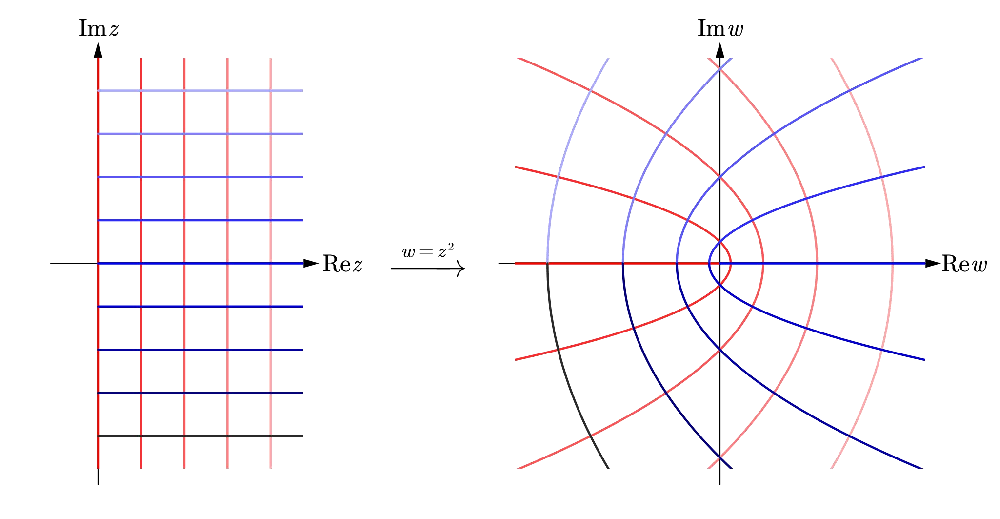
\includegraphics[scale=0.75]{map_z.pdf}
    \caption{映射$w=z^2$将右半复平面映成几乎整个复平面}
\end{figure}


复变函数的级数部分讲的主要是Taylor级数和\uwave{Laurent级数}。解析函数的Taylor级数与实函数部分差别不大,但是由此直观地审视了“收敛圆”的概念,并且考察复变函数对考虑实函数级数的收敛域是有帮助的。一个经典的例子是$f(x)=\dfrac{1}{1+x^2}$,在实轴上看该函数处处都是任意阶可导的不存在极点;而在整个复平面上看,它有两个极点$\pm\mathrm{i}$,于是在$0$处展开时该级数的收敛半径为$1$。Laurent级数是对Taylor级数的推广,允许级数中存在负幂次项。对于极点数目有限的函数,Laurent级数至少能够对一个圆环区域收敛,这就允许我们考察在极点处的函数展开,例如余割函数$\csc z$在$z=0$处的展开:
\[
    \csc z=\frac{1}{z}+\frac{z}{6}+\frac{7z^3}{360}+\cdots
    .\]
\uwave{Z变换}与Laurent级数紧密相连,Z变换在处理离散序列信号,以及解差分方程中发挥重要作用。

复变函数的积分部分的内容十分精彩,可以说复变函数成为一个相对独立的数学分支与这一部分的结论分不开。借助Green公式,能够证明\uwave{Cauchy积分公式}和闭路变形定理,将解析复平面上的环路积分归结成极点附近积分的计算,这里会考察极点的性质以及\uwave{留数}。随后还有将导数与积分建立起联系的Cauchy积分公式,这为级数中系数的计算提供了另一种手段。

有些教材会在后边附上关于\uwave{Fourier变换}和\uwave{Laplace变换}的内容,也有课程安排将这两部分放到数学物理方程中去讲。所谓积分变换,是将一个变换$\mathscr{T}$作用在一个函数$f(t)$上获得另一个函数$F(p)$的过程:
\[
    F\left( p \right) =\mathscr{T}\left[ f\left( t \right) \right] =\int_a^b{f\left( t \right) K\left( t,p \right) \,\mathrm{d}t}
    .\]
而新函数$F(p)$中包含了原函数$f(t)$的信息,从而转换了对于一个函数的研究视角。根据所选的变换核函数$K(t,p)$的形式,将积分变换分成不同种类,如选择$K(t,\omega)=\mathrm{e}^{-\mathrm{i}\omega t}$得到Fourier变换,选择$K(t,s)=\mathrm{e}^{-st}$得到Laplace变换等。


Fourier变换是从Fourier级数引入的,Fourier级数考察的是周期函数中一个有限的区间,Fourier变换考察的是任意函数(要求绝对可积),而非周期函数可以看作是周期无穷大的周期函数,所以能够通过Fourier级数引入Fourier变换。不同学科中对Fourier变换的定义是略有区别的,有些地方可能差一个常数倍,讨论之前需要注意。如果不引入广义函数$\symup\delta(t)$,像$1,\sin t,\cos t$这样简单的函数都是没法做Fourier变换的。但是注意,这当中的广义函数如冲激函数$\symup\delta(t)$、阶跃函数$H(x)$其实并不是函数,由于所学知识有限,不会对更本质的内容做过多的探讨,但是一定注意其与我们传统意义上的函数之间的区别。例如,涉及到$\symup\delta(t)$的导数的一定是弱导数,而不是经典意义下的导数,在使用时务必要遵循我们事先约定好的定义。Fourier变换在求解微分方程以及信号的频谱分析等方面有重要作用。

Laplace 变换是将算子法解微分方程严密化而来的。Laplace 变换没有像 Fourier 变换那么多需要注意的坑,记好基本内容就够用了。这里多提一点Fourier变换和Laplace变换为何能在解微分方程中发挥作用,这是这两种变换的微分与积分性质决定的,这两种变换能够将微积分这两种分析学运算转化成乘除法这样的代数运算,从而在形式上简化了求解过程。那么,问题一定变得简单了吗?不一定,因为这个过程实际上将复杂的计算转移到了求变换与逆变换的过程中了,如果有完善的积分变换表可以查询,那么问题确实简单不少。这个过程就好像人们曾经为了简化大数乘法而发明对数,将乘法转化成加法一样,形式上问题简化了,但是复杂的计算被隐藏到了求对数这一过程中。

\paragraph{与力学专业内容的联系}

\begin{itemize}
    \item 离散信号分析、差分方程求解——Z变换,实际上就是Laurent级数

    \item 连续介质力学平面问题中,关于有势场散度的描述——解析函数的实部和虚部均为调和函数

    \item 二维弹性问题求解、无限大平板圆孔问题、断裂力学三类基本裂纹求解——弹性问题的复变函数解法
\end{itemize}

\paragraph{学习建议}

复变函数部分,类似微积分,以熟悉基本的运算规则和定理公式为主,但没必要做太多奇怪的计算,我们直接用到复变函数计算的内容其实不多,熟悉常用的几类计算即可。重点可以放在积分变换部分,主要去熟悉积分变换的基本性质,为后续解微分方程服务。Fourier变换可以额外留意一下,力学中的实验手段或是一些处理微分方程的问题中,Fourier变换是十分常用的,务必要将所有概念牢牢掌握。

\paragraph{参考书目}

\begin{center}
    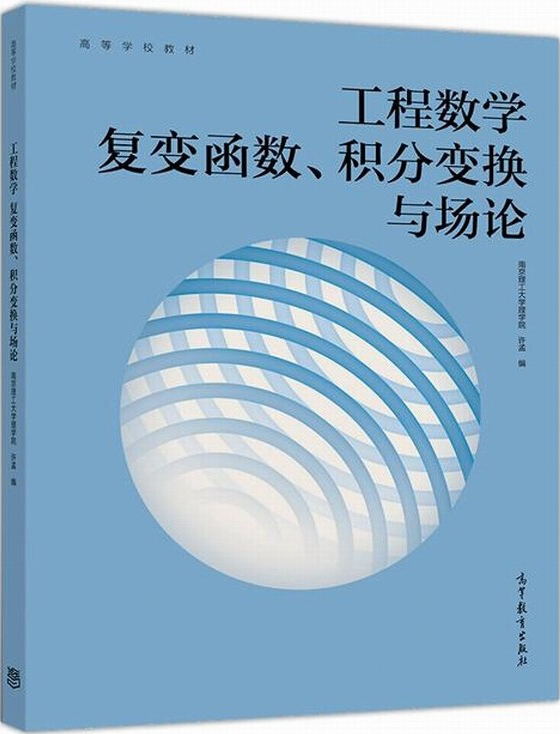
\includegraphics[scale=0.38]{book/9.png} \quad
    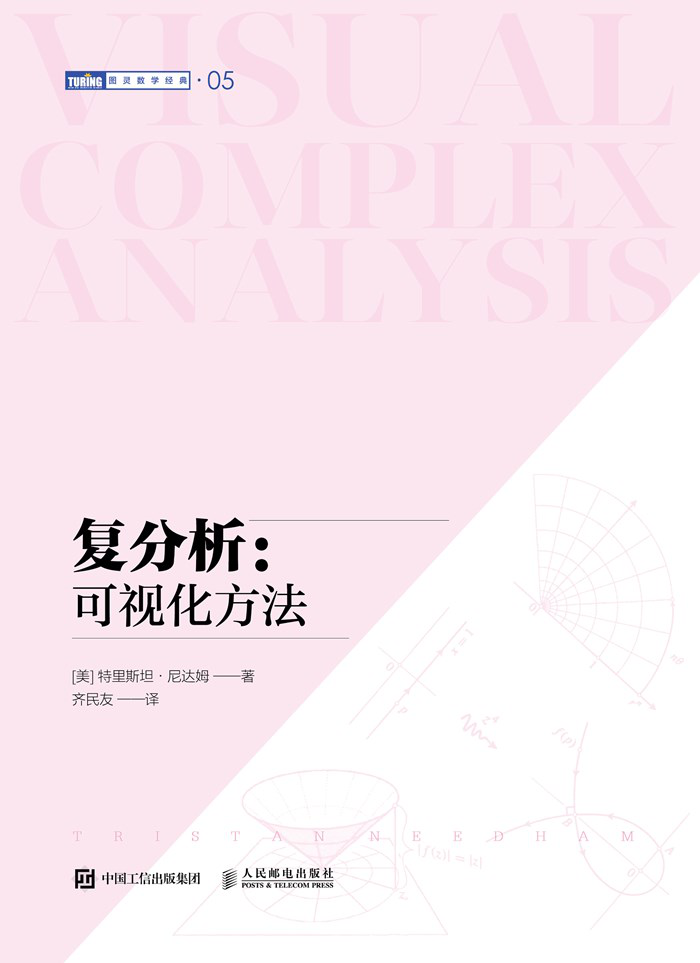
\includegraphics[scale=0.23]{book/10.png}
\end{center}

\begin{itemize}
    \item \textcite[工程数学——复变函数、积分变换与场论]{工程数学——复变函数、积分变换与场论}

          这本教材的优势在于对于前两章的基础处理比较细节,在此处也直接引入了对保形映射的讨论,几何直观性做的比较好。此外,在积分变换部分,这本书给出了对Mellin变换、Hankel变换和Z变换的内容,这些变换在特定的场合能够发挥作用,可以作为补充材料有针对性地学习。

    \item \textcite[复分析:可视化方法]{needham2009复分析可视化方法}

          这本教材从几何直观的角度讲解复变函数,同时内容没有超出我们一般所学的复变函数的内容太多,可以满足几何可视化的需求。该书内容较多,不必通读,建议有选择、有针对性地读。
\end{itemize}

\subsubsection{数学物理方程}

\paragraph{前置知识}微积分、线性代数、积分变换

\paragraph{部分知识介绍}

这门课的内容概括起来就是:如何解二阶线性偏微分方程的定解问题。

首先会了解一些偏微分方程中的基本概念,以及从一些常见的数学物理问题中提炼出不同的二阶线性偏微分方程,其中一些具有共同形式,于是将其大致分类为\uwave{椭圆型}、\uwave{抛物型}与\uwave{双曲型}:

\begin{itemize}
    \item 椭圆型:$\Delta u = f$.
    \item 抛物型:$\dfrac{\partial u}{\partial t}-k\Delta u = f$.
    \item  双曲型:$\dfrac{\partial^2 u}{\partial t^2}-a^2\Delta u = f$.
\end{itemize}

其中$\Delta=\displaystyle\sum_{i=1}^{n}\dfrac{\partial^2}{\partial x_i^2}$是Laplace算子,$u$是未知函数。这个名字由来与对曲面上一点的类型相似,都来源于对系数矩阵特征值的讨论。不同类型的方程具有不同的性质,分门别类地讨论是很有好处的。

\begin{figure}[ht]
    \centering
    \begin{subfigure}[t]{0.3\textwidth}\centering
        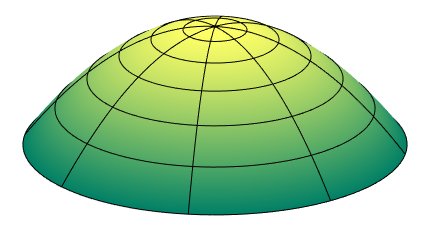
\includegraphics[height = 0.5\linewidth]{ellipse.png}
        \caption{椭圆点(两特征值同号)}
    \end{subfigure}
    \begin{subfigure}[t]{0.3\textwidth}\centering
        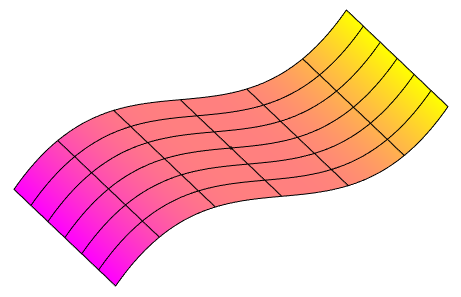
\includegraphics[height = 0.5\linewidth]{parabolic.png}
        \caption{抛物点(一特征值为零)}
    \end{subfigure}
    \begin{subfigure}[t]{0.3\textwidth}\centering
        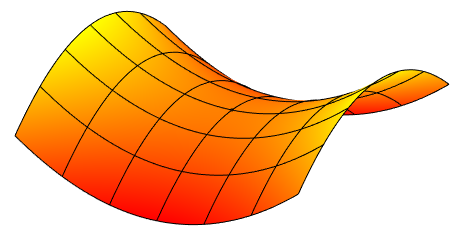
\includegraphics[height = 0.5\linewidth]{hyperbolic.png}
        \caption{双曲点(两特征值异号)}
    \end{subfigure}
    \caption{按特征值对三类点进行分类}
\end{figure}

解偏微分方程与解常微分方程的不同之处在于,假设方程的形式比较好,可以直接积分,那么常微分方程做一次积分会出现一个待定的任意常数,而偏微分方程做一次积分会出现一个待定的任意函数,这时二者最根本的区别。所以对偏微分方程作积分最多能得到形式上的解,有的时候可以根据初始条件或边界条件确定解的具体形式,然而更多的时候是没法确定的,退一步讲有些形式解还包含复数,从而引起很复杂的讨论,更何况能直接作积分的偏微分方程更是少之又少。

这门课中处理线性偏微分方程的手段一般有三种:级数法(分离变量)、积分变换法和\uwave{Green函数}法,这些方法能用的原因与方程解的线性性有关。所以这门课的讨论事实上并不复杂。

级数法首先假设解函数可以写成若干一元函数之积的形式,如对于 $u = u (x,y)$,通常假设$u(x,y)=X(x)Y(y)$(能够证明这样假设是合理的),随后通过选择一个合适的函数列(一般而言是一个可列无穷多的序列),将解表示为这个函数列的线性组合。最常用的函数列是Fourier级数,但对于不同形状的区域来说,这个函数列的选择一般是不同的。至于这个函数列如何选取,还要用到\uwave{Sturm–Liouville方程}的相关理论,同时涉及到一些特殊函数的知识。

从Fourier级数引入Fourier变换的思想也可以用在这里。级数法处理的都是有限区域,对于半无界或无解区域就要用到积分变换法了。并且类似级数法,当使用不同形状的坐标系考察问题时,用到的积分变换可能也是不同的。

Green函数法具有深厚的物理背景,它从考虑点电荷场分布的问题而来。直观地说,如果我们知道点源产生的场的分布情况,就能通过对研究区域进行线性叠加,找到一个满足给定定解条件的方程的解,这个点源的分布函数就是Green函数。所以,如果能找到某一个问题相应的Green函数,这个问题就好解决了。Green函数不仅与方程的形式有关,与边界条件也有关,甚至与问题的维数也有关。

\paragraph{与力学专业内容的联系}

\begin{itemize}
    \item 诸多椭圆型微分方程的求解(弹性力学中的静力学问题、模态分析等)——基于分离变量法的Fourier级数解法

    \item 边界元法方程构建——Green函数法
\end{itemize}

\paragraph{学习建议}

一般来说,这门课的起点不会太高,甚至有些学校的数学物理方程这门课被称为“微积分习题课”都不夸张,但如果能够多学一点,这门课还是很实用的。这门课的一大特点是,理论不复杂,看起来好像很好处理,但其中涉及到的细节很多,所以最好将学习过程中涉及到的计算、推导流程操作一遍。另外,这门课中会接触到许多来自物理学和力学的模型,积累一些模型及相应方程是很有好处的。

不过,得益于各类计算机硬件条件和数值计算方法的发展,以及出于对非线性方程求解的需求,求解析解似乎变成了一个有些费力不讨好的事情。但不论如何,解析求解都应该是理论工作者应当追求的东西。而且这门课中学习的处理手法都是比较基础和简单的,有些思路或理论在构建数值算法时也会用到,所以掌握这些内容还是很有必要的。

\paragraph{参考书目}

\begin{center}
    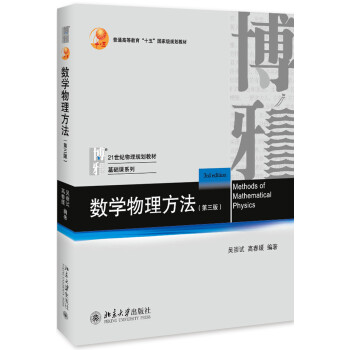
\includegraphics[height = 6cm]{book/11.jpg} \quad
    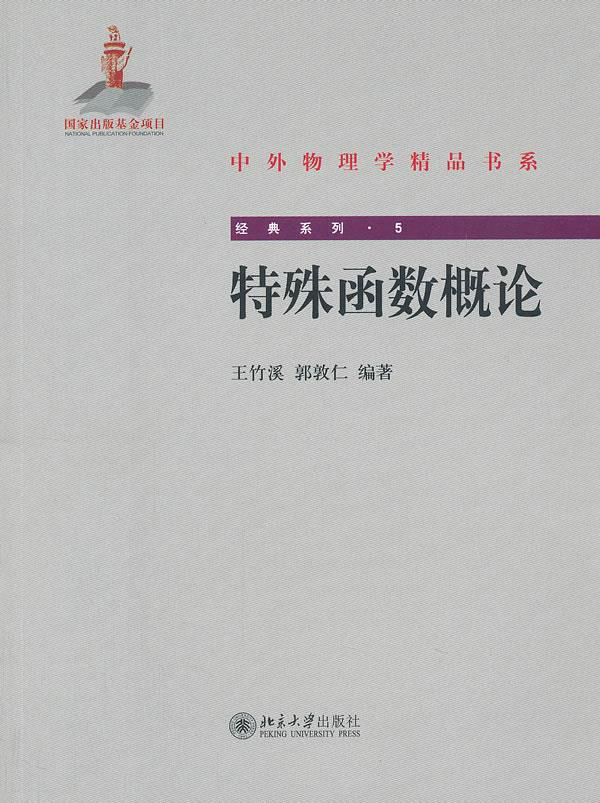
\includegraphics[height = 6cm]{book/12.png}
\end{center}

\begin{itemize}
    \item \textcite[数学物理方法(第3版)]{数学物理方法(第3版)}

          这本书的内容十分丰富,前一部分非常详尽地讨论了复变函数、积分变换和特殊函数的理论,这一部分也可以作为复变函数部分学习的参考资料。后一部分则是解线性偏微分方程的内容,相比于大多数国内教材,这本教材将数学方程与物理背景的联系比较好,对于各类具体形式的方程及其边界条件的讨论也比较详尽。此外,这本书还简单地介绍了变分法,变分法在理论分析和计算上的用处都很大,后边还会介绍。

    \item \textcite[特殊函数概论]{特殊函数概论}

          特殊函数的研究内容十分宽泛,但我们只需要关注在解一部分方程的过程中出现的特殊函数就足够了。这本书的一二章介绍了级数和二阶常微分方程的基本理论,第三、五、七章分别介绍了$\Gamma$函数、Legendre函数和Bessel函数这几类在物理方程中经常出现的特殊函数。由于处理特殊函数的技巧性很强,所以在数值解出现之后人们往往也就不那么关注特殊函数解了,但在有些时候分析问题的性质时还是有用的。这本书本身可以作为工具书使用,查询一些特殊函数的特定性质。

    \item \textcite[积分方程(第3版)]{积分方程(第3版)}

          讲授积分方程求解的课程和参考书很少,这本书是少有的详细讲解积分方程求解的参考书,而且没有用到太高深的数学概念。积分方程有很多实际应用的情景,许多物理和力学问题都需要用积分方程描述,积分方程相较于微分方程有一个好处,就是降低了对解可微性的要求。此外,学习积分方程也可以为泛函分析提供学习的实例与动机。

          \begin{center}
              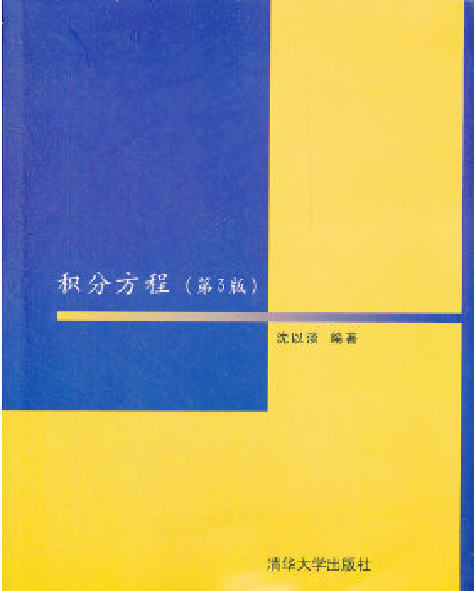
\includegraphics[scale=0.59]{book/13.png} \quad
              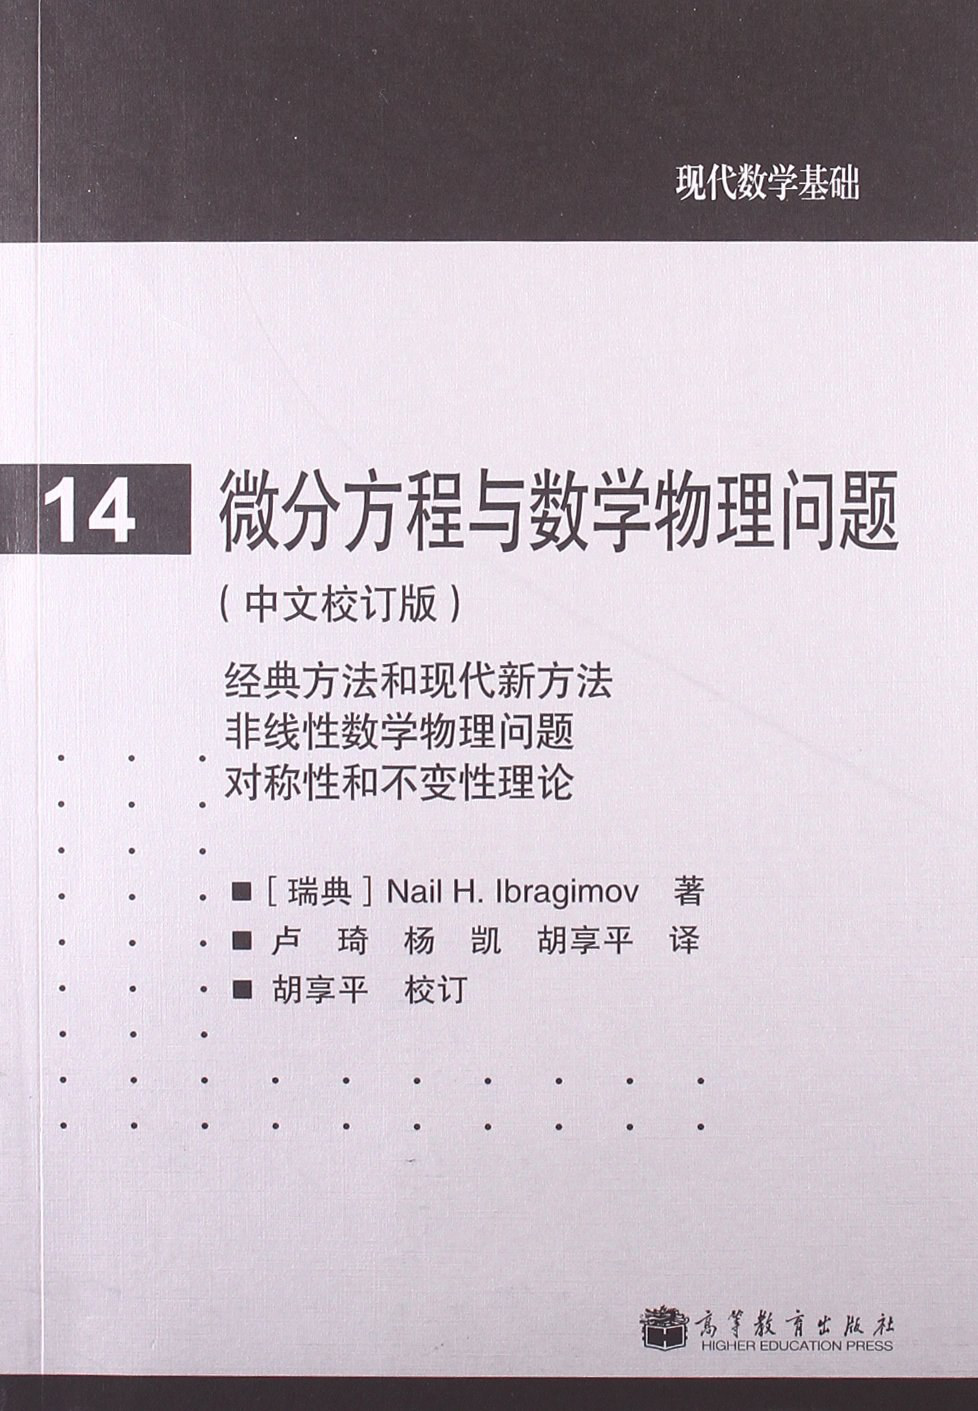
\includegraphics[scale=0.2]{book/14.png} \quad
              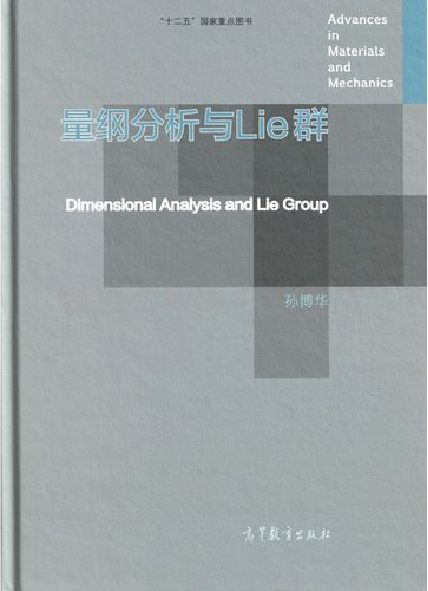
\includegraphics[scale=0.59]{book/15.png}
          \end{center}

    \item \textcite[微分方程与数学物理问题]{ibragimov2013微分方程与数学物理问题}

          这本书的前五章大致是经典的处理线性微分方程的理论,其中的亮点是物理模型比较丰富,以及介绍了一阶偏微分方程的理论。后半部分从对称性(Lie群)的工具探讨了非线性方程的处理方法,对用解析手段处理微分方程感兴趣的读者可以将其作为拓展阅读材料。

    \item \textcite[量纲分析与 Lie 群]{孙博华2016量纲分析与Lie群}

          量纲分析是处理力学问题当中常用的一种技巧,而量纲分析与Lie群存在联系。这本书还比较细致地介绍了用Lie群工具处理微分方程的基本理论和具体算法。另外,这本书中涉及到的物理模型也是比较丰富的。

\end{itemize}

\subsubsection{数值分析}

\paragraph{前置知识:}微积分、线性代数

\paragraph{部分知识介绍}

很多问题的解析求解是十分困难的,甚至是不可能的,所以在大多数时候,我们只能退而求其次,去寻求程序化的近似解。同时,计算机的发展对于程序化求近似解来说无疑是一个好消息,但计算机没法直接处理涉及无穷的问题,所以发展各种离散的近似算法就是十分必要的。这就是数值分析所做的工作,除了构建算法,还需要研究这些算法的可靠性,具体地说,有算法\uwave{效率}、\uwave{稳定性}分析、\uwave{误差}分析。

数值分析课程大致可以分成三部分,一是数值代数,二是数值逼近,三是常微分方程数值解。数值代数中一般包含以下内容:非线性代数方程求解、线性方程组求解和矩阵特征值求解;数值逼近中一般包含以下内容:\uwave{插值}、\uwave{逼近}与\uwave{拟合}和数值积分。这门课程的特点是内容多而杂,但实用性很强。

数值代数的主要任务是解方程和处理矩阵。首先是解非线性代数方程,三次、四次方程根式解的形式已经十分复杂,而五次及以上方程和一般的超越方程更是没有根式解,所以用数值方法求一般的非线性代数方程的近似解就很必要了。大规模的线性方程组按Gauss消元求解,它可以归结为直接\uwave{分解法},另一种常用的方法是\uwave{迭代法}。它们的构造与分析主要用到矩阵理论,主要包括矩阵分解和范数计算。矩阵特征值的求解没有什么需要强调的。一个比较有意思的点是,求解多项式方程时,因为Frobenius矩阵特殊的形式,它的特征值求解等价于一个多项式方程的求解,该方法能得到多项式的所有根,而不像迭代法只能求得一个根。


\begin{figure}[ht]
    \centering
    \begin{subfigure}[t]{0.45\textwidth}\centering
        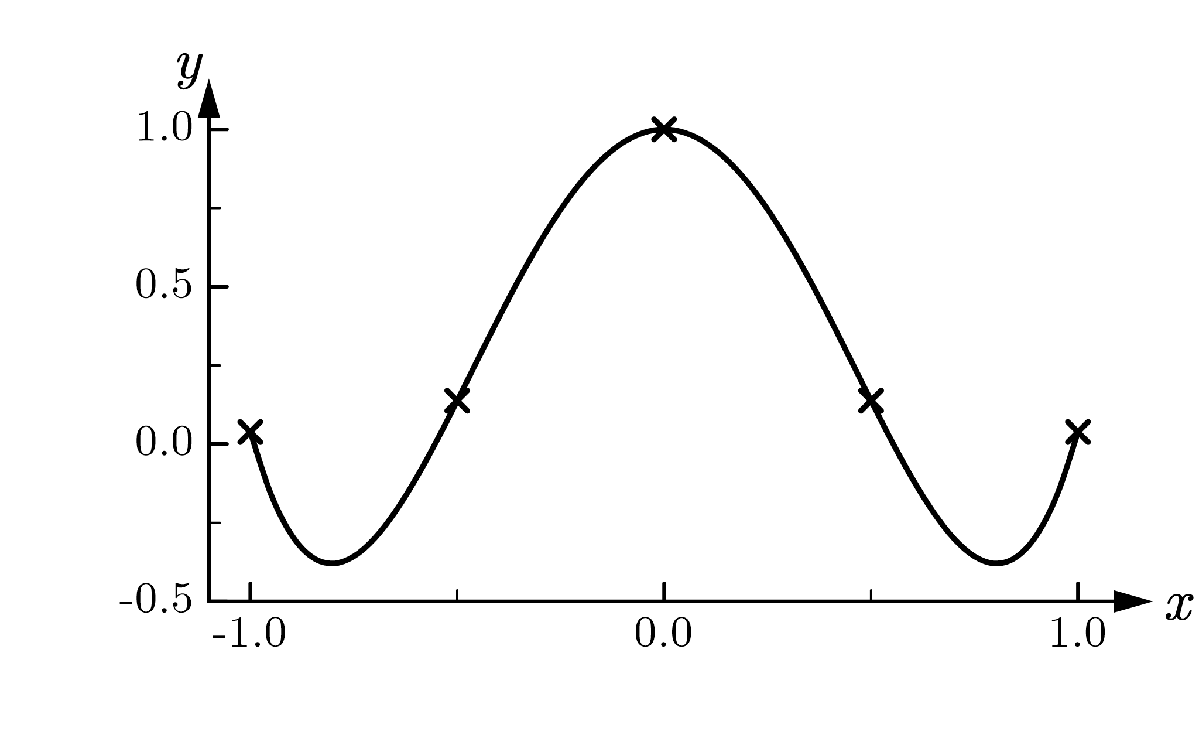
\includegraphics[height = 0.55\linewidth]{interpolation.pdf}
        \caption{插值}
    \end{subfigure}
    \begin{subfigure}[t]{0.45\textwidth}\centering
        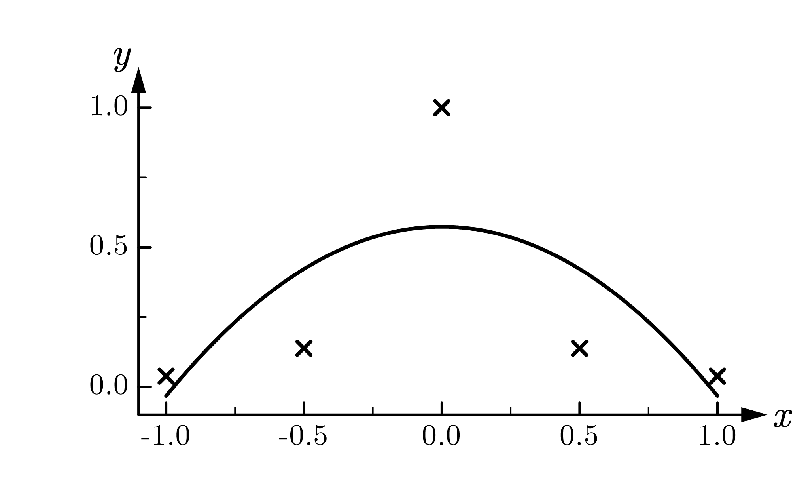
\includegraphics[height = 0.55\linewidth]{fitting.pdf}
        \caption{拟合}
    \end{subfigure}
    \caption{插值与拟合的联系与区别}
\end{figure}

\begin{figwindow}[2,r,
        {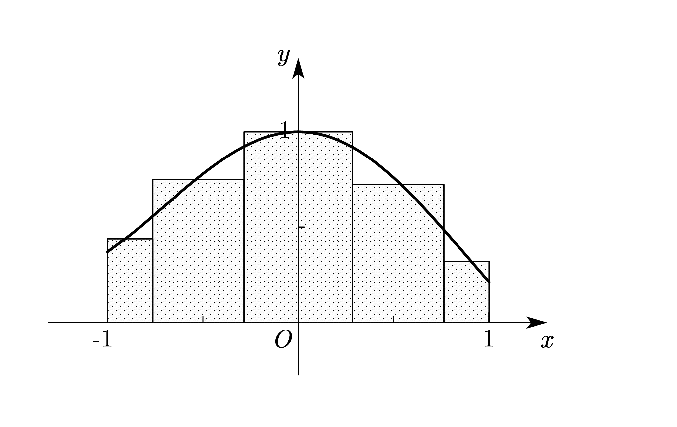
\includegraphics[scale=0.7]{numerical_integration.pdf}},
        Gauss-Legendre求积公式示意]
    数值逼近的主要研究如何找到一个函数使得它跟已知函数或若干已知点“最接近”。插值、逼近和拟合的概念比较相似,但又有一定的区别。插值、逼近和拟合都是用一组函数的线性组合来近似一个函数关系,区别在于,插值和拟合问题要逼近的是若干数据点,且插值要求待求函数通过给定的数据点,拟合则不需要;逼近则是寻求与已知函数最接近的函数。由于插值通过所有已知数据点,所以它天然就满足“最接近”的要求,逼近和拟合中则要定量描述“最接近”。在此以前,我们接触的描述接近程度的工具,也就是距离,都是针对数或者点来说的,而此处的距离则是针对函数提出的。这里概念的推广需要转换一下脑筋,将函数视为一种向量,而一组基函数张成一个有限维线性空间,同时,这个线性空间上往往又拥有“距离”、“内积”的概念(请回忆在线性代数部分提过的类比!),我们就可以在这个十分类似于欧氏空间的线性空间上讨论问题。这样,研究对象就很接近线性代数中的内容了,也容易从几何直观上考虑问题。数值积分的方法十分朴素,其思想就是还原了用Riemann和定义积分的方法,因此这一部分就不展开介绍太多了。只提两个比较有用的算法,一是\uwave{Gauss求积}方法,这种方法的代数精度比较好,因此应用较多;二是Romberg算法,它能加快收敛速度,且具有稳定性好的优点,同时这种思想也能推广到一些其它的数值计算方法上。
\end{figwindow}

解常微分方程部分一般讲的是\uwave{有限差分法}(FDM)格式的构造,在构造差分格式时,用得比较多的是Taylor展开和数值积分公式两项技术,在求解时往往还要涉及到大规模线性方程组求解,所以前边学的方法在这里都能用上。解常微分方程最常用的方法是\uwave{Runge-Kutta方法},该方法的收敛效果一般都比较好,目前已经在很多领域得到应用。

\paragraph{与力学专业内容的联系}

\begin{itemize}
    \item 可以说,如今的力学领域从事与计算相关的研究很多,所以数值方法与力学问题的求解是广泛相联系的。这里只举一些例子:

    \item 数字信号分析——快速Fourier变换

    \item 模态分析的数值解法——矩阵特征值的数值解

    \item CAD当中的B\'ezier曲线——基于Bernstein多项式的插值
          \begin{figure}[ht]
              \centering
              \begin{subfigure}[t]{0.45\textwidth}\centering
                  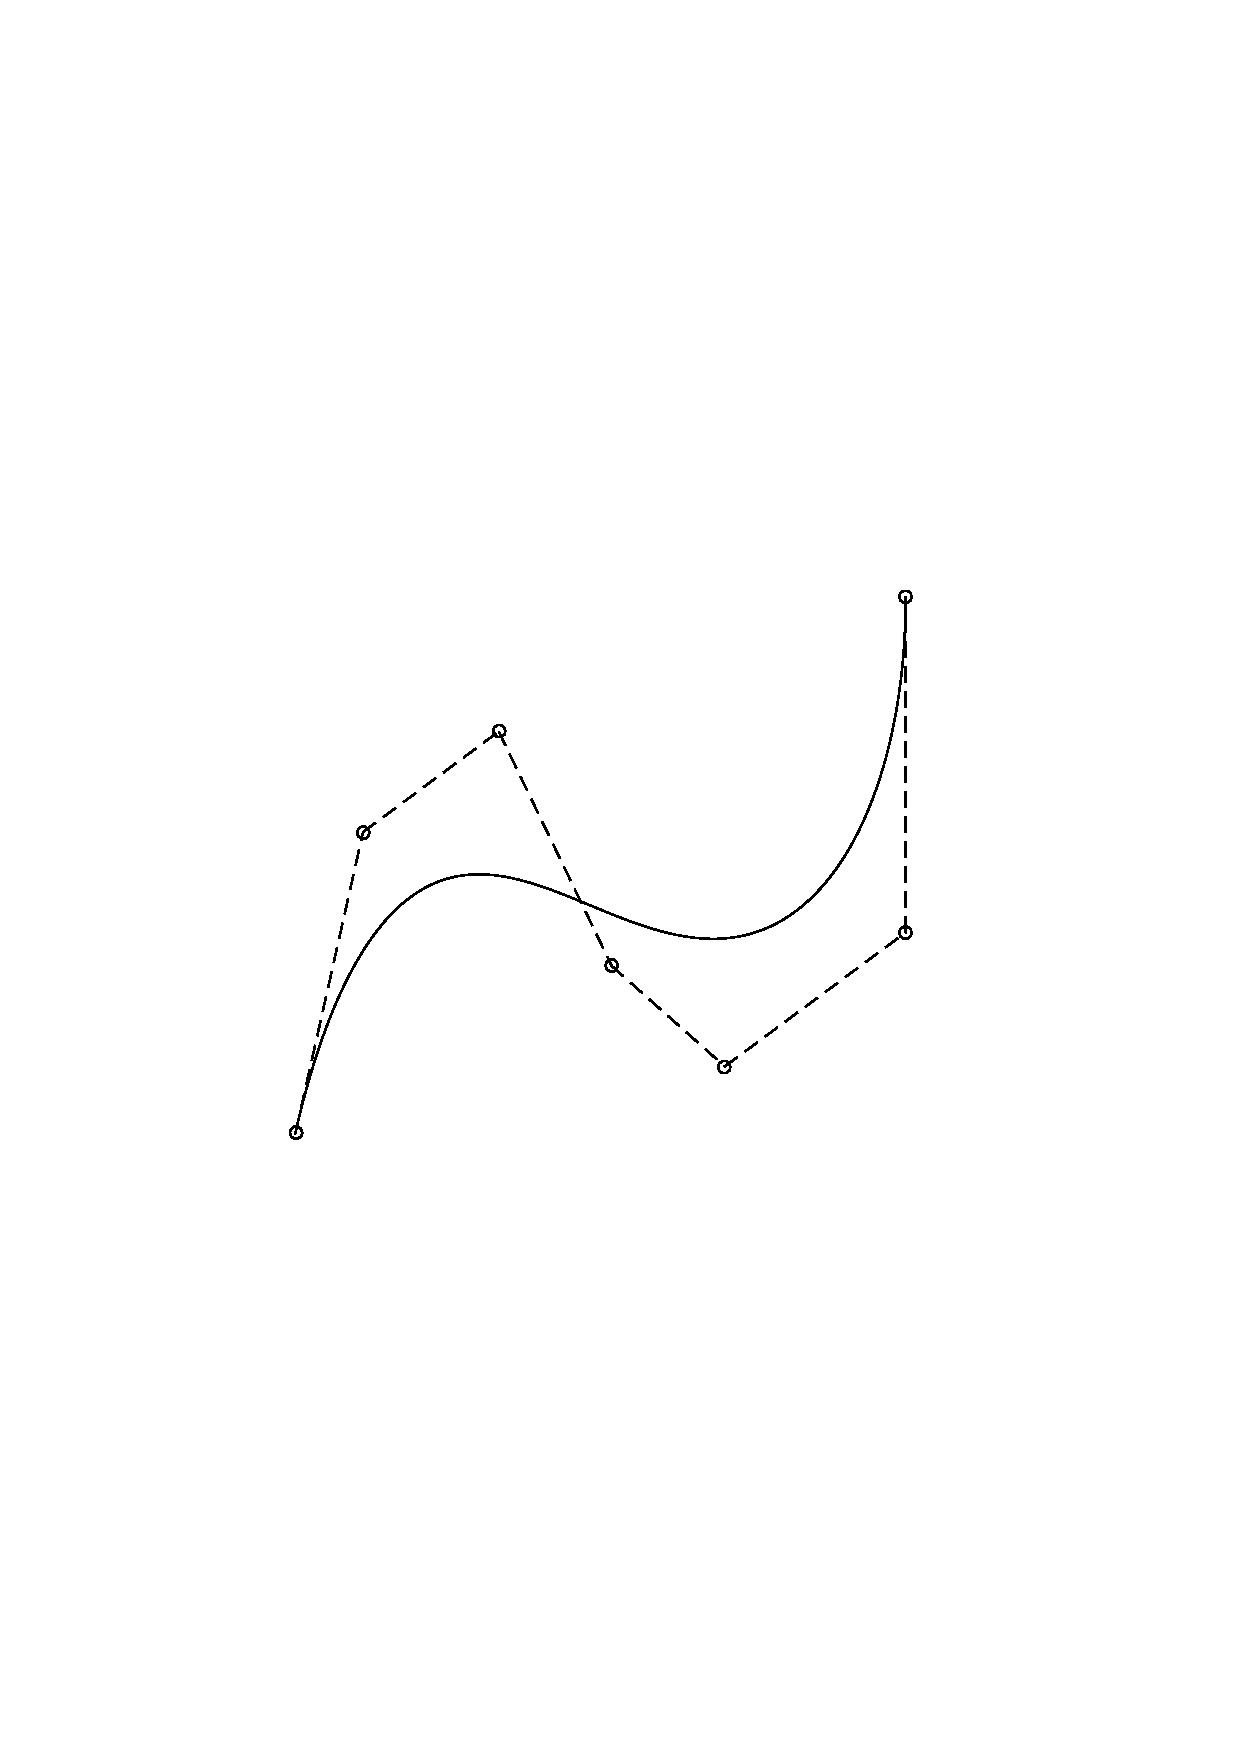
\includegraphics[height = 0.55\linewidth]{beizer.pdf}
                  \caption{$6$次B\'ezier曲线  }
              \end{subfigure}
              \begin{subfigure}[t]{0.45\textwidth}\centering
                  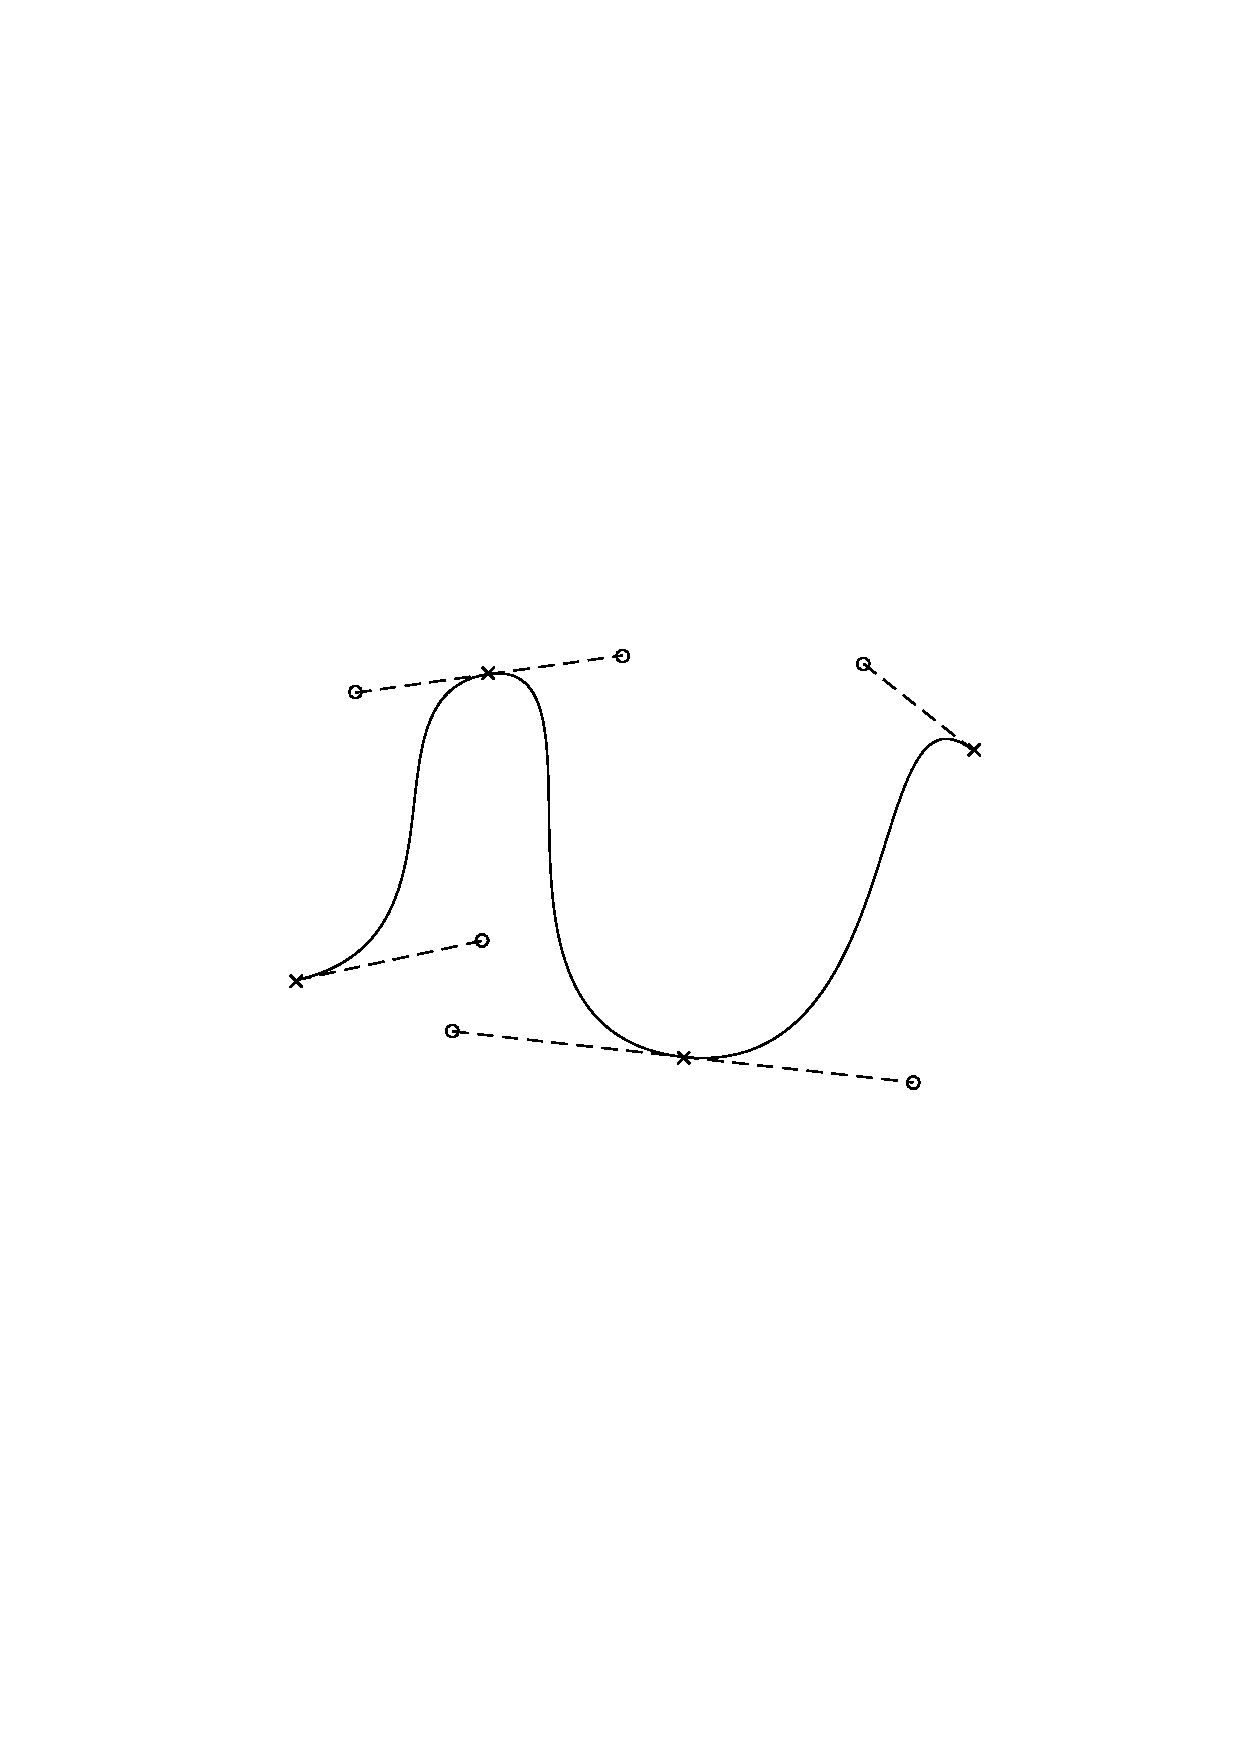
\includegraphics[height = 0.55\linewidth]{beizer3.pdf}
                  \caption{分段光滑$3$次B\'ezier曲线}
              \end{subfigure}
              \caption{B\'ezier曲线示例}
          \end{figure}
    \item 有限元法中形函数的构建——Lagrange插值

    \item 有限元法中对积分的处理——Gauss积分公式

\end{itemize}
\paragraph{学习建议}

数值分析这门课不只要学习理论,更要注意编程实现一些重要的算法。尽管诸如MATLAB等数学软件中已有现成的函数可以直接调用,但在初次学习时还是应该手动编程实现整个过程,一方面加深对算法的理解,另一方面也可以锻炼自身的编程能力。

此外,可以阅读 \textcite[数值泛函及其应用]{张维强2021} 的前四章,这一部分讲了数值分析中一些来源于泛函分析的概念,可以了解一些概念的定义以及常用定理,将一些问题纳入赋范线性空间下直观地考虑。

\paragraph{参考书目}

\begin{figure}[h]
    \centering
    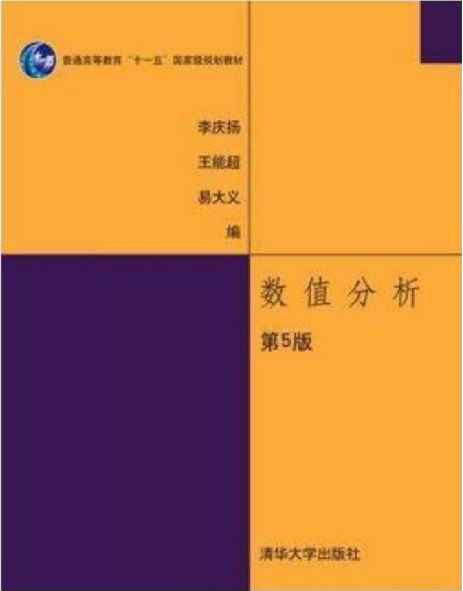
\includegraphics[scale=0.6]{book/16.png}
\end{figure}

\begin{itemize}
    \item \textcite[数值分析]{李庆扬2009}

          这本书的内容相当丰富,涵盖了签署的所有内容,并且内含一些拓展内容及实用的算法,如快速Fourier变换等。不过该书没有代码示例,可以参考一些算法实现集,或者在互联网上寻找。
\end{itemize}



\subsection{后续及定向数学培养简介}

上述进阶培养的内容对于本科阶段的专业课来说基本够用了,但是也有一些针对特定方向,以及满足更深入学习需求的数学课。因为这些内容已经超出新生所能接触到的数学很多了,所里这里我们只简单介绍一下,更详细的信息请有兴趣或需要的读者自己查阅资料。

总体来说,力学所研究的问题都围绕“如何建立描述力学问题的方程”和“如何求解方程”展开,因此延续了以分析学为主的画风。\autoref{fig:力学系的数学科技树} 中画虚线框的课程是不必掌握的,很多学校的力学专业也不一定开设,可以在有需要的情况下按照科技树的路线自行学习,当然,科技树的路线不是死的,有些前置知识的缺失可能对后续内容的学习影响不大,请做好取舍。下面粗略地介绍一下力学当中几大主干大致需要的数学基础。

\paragraph{常微分方程}

\begin{figure}[h]
    \centering
    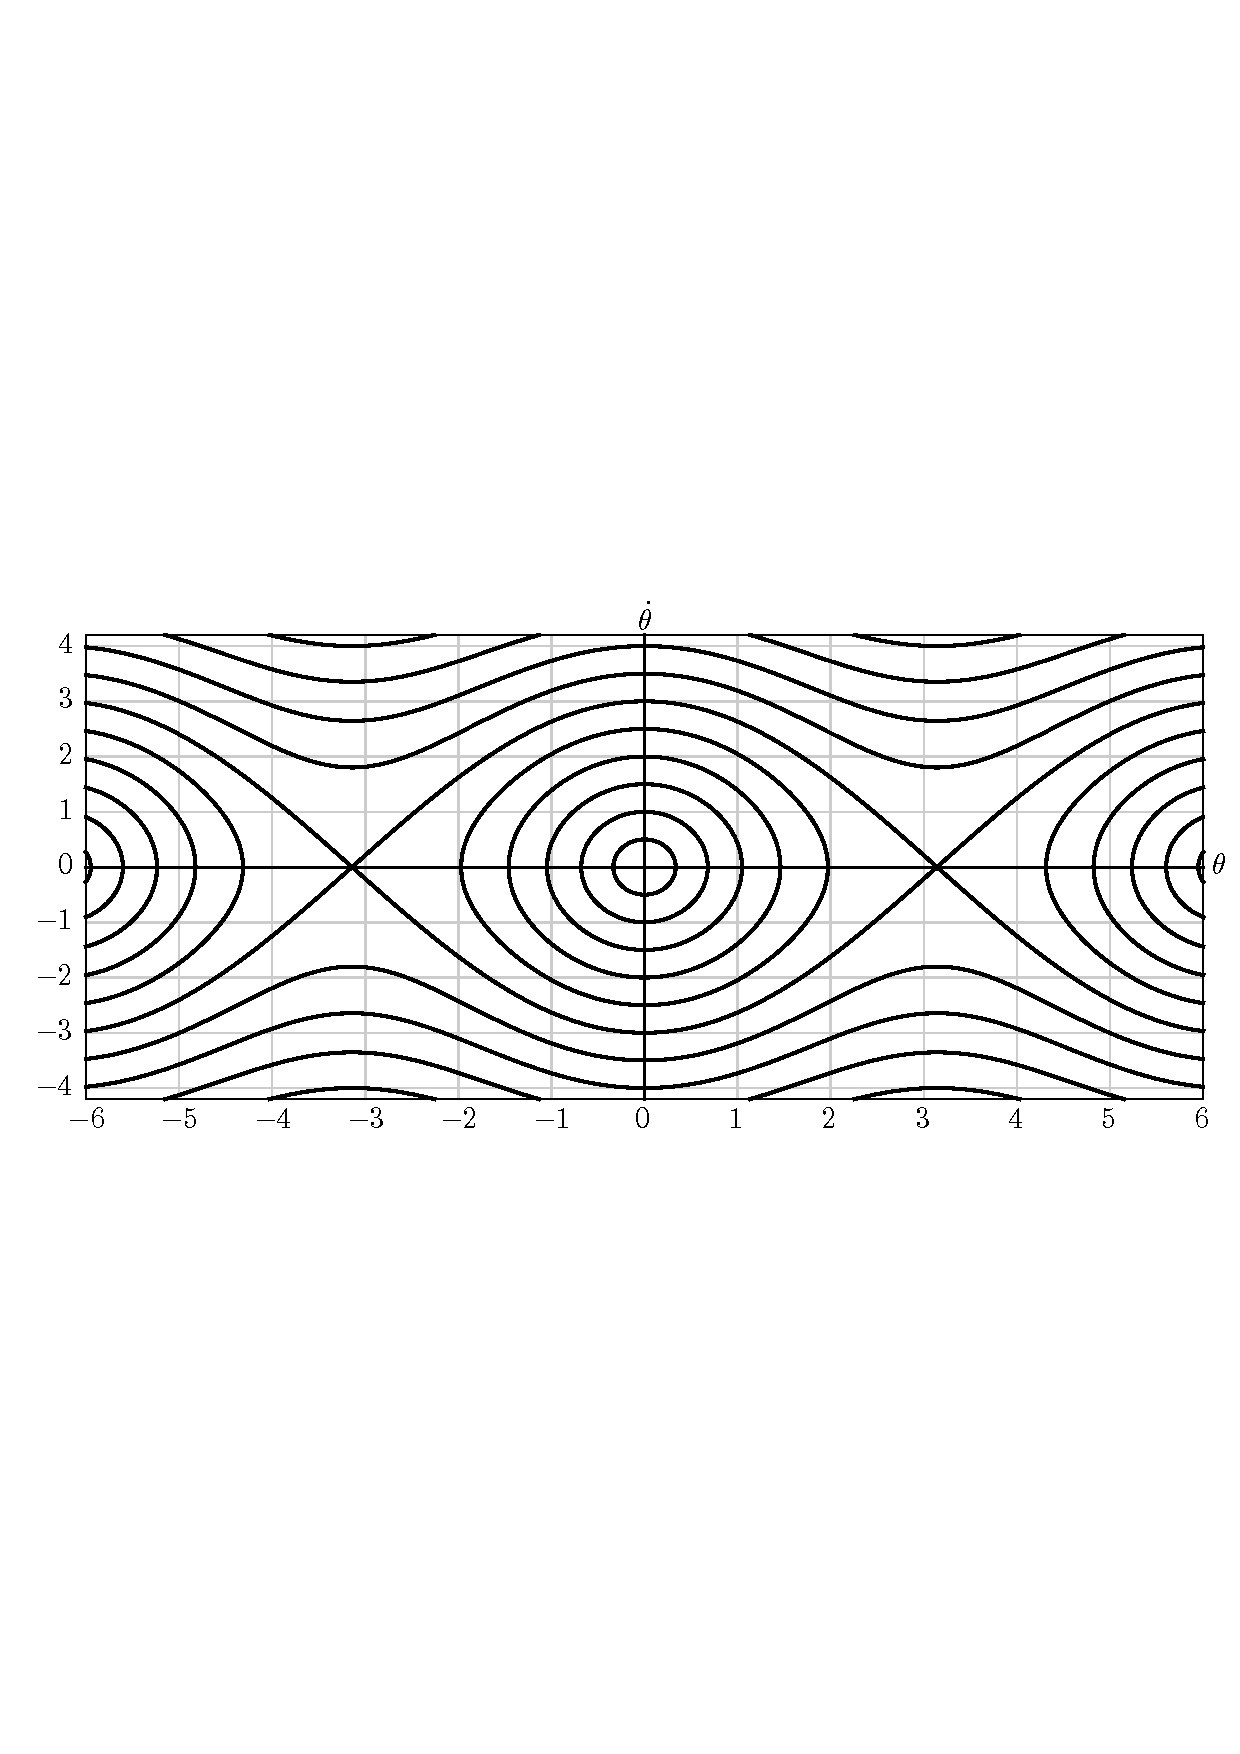
\includegraphics[scale=0.65]{phase.pdf}
    \caption{单摆的相空间曲线图}
\end{figure}

常微分方程在微积分中讲过一些内容,在此基础上,可以学习这些内容:一阶微分方程解的性质、非线性微分方程的定性分析、微分方程的级数解、一阶线性偏微分方程和边值问题。

对一阶微分方程解的性质的研究为数值方法提供了理论基础;一阶线性偏微分方程和边值问题可以选择在开设数学物理方法之前学习一下,与特征线相关的理论在数学物理方法中有直接的应用。对于一般力学方向来说,最重要的则是微分方程的定性分析,其中诸多概念与理论在动力学及控制中是十分基础的,并且有广泛的运用。

\paragraph{参考书目}

\begin{figure}[h]
    \centering
    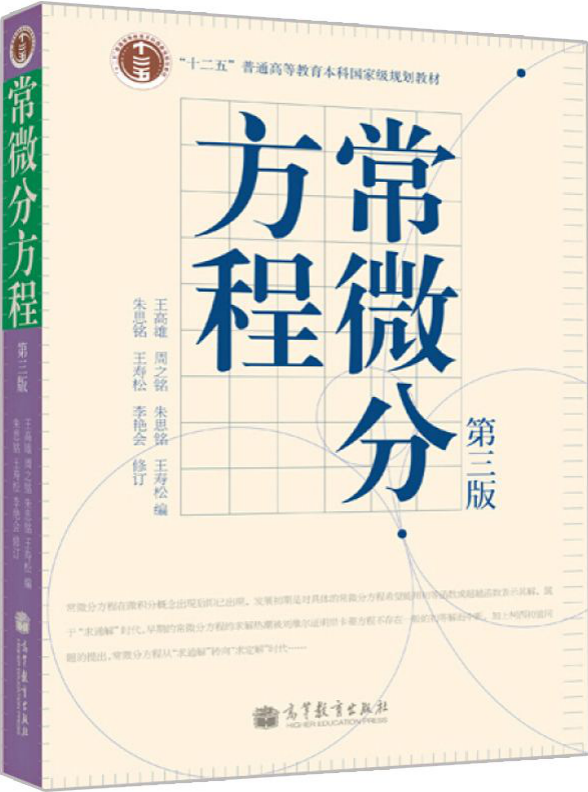
\includegraphics[scale=0.36]{book/17.png}
\end{figure}

\begin{itemize}
    \item \textcite[常微分方程(第四版)]{王高雄2020常微分方程}

          这本书涵盖了前边的大部分内容,并且所讨论的数学理论不算太深,作为入门级基础读物很适合力学专业的同学们。
\end{itemize}

\paragraph{矩阵分析}

矩阵分析基本上是线性代数的升级版,约等于数学系的高等代数这门课,但不太涉及多项式理论。从实用角度来说,线性代数部分的理论和计算实际上是不太够用的,一些比较关键的问题处理的概念思路可能也是要在矩阵分析中才能遇到。

矩阵分析这门课大致可分成几个部分:一是矩阵的标准型及分解,二是矩阵的微积分,三是矩阵方程的求解。另外,这门课一般默认在复数域$\mathbb{C}$中考虑问题。

在介绍矩阵的标准型和分解之前,这门课一般都会补充线性代数中被忽略掉的\uwave{线性空间}的基本理论,有了线性代数等前置课程做基础,理解线性空间和线性映射会更加得心应手。矩阵标准型部分最重要的就是\uwave{Jordan标准型},由于它能处理任意矩阵高阶幂问题,所以它是矩阵微积分中很多重要理论的基础。矩阵分解部分最重要的是\uwave{奇异值分解}和\uwave{极分解},奇异值分解应用很广,最著名的便是主成分分析;极分解提供了一个很典型的几何直观的例子,它将一个一般的线性变换分解为旋转变换与伸缩变换的复合,这在连续介质力学中能找到很好的对应。

矩阵微积分讨论的是矩阵函数及其微积分。在讨论微积分之前,首先一定要有\uwave{度量}这个概念,在此基础上才能进一步引入微积分中的极限、收敛、连续等概念,进而讨论微积分。矩阵的“度量”便是\uwave{范数},范数是绝对值或模长概念的推广。对于有限维线性空间来说,矩阵按范数收敛和矩阵收敛是一回事,于是矩阵范数就给讨论矩阵微积分打下了基础。此处还有一个相当关键的定理——\uwave{Hamilton-Cayley定理},这条定理保证了:对于$n$阶方阵$\symbfit{A}$,其矩阵函数一定能用$\symbfit{A}$的不超过$n$次幂的线性组合表出,从而大大简化了矩阵函数的计算。

矩阵方程不一定限于$\symbfit{Ax}=\symbfit{b}$这种简单的形式,称如下的代数方程组(或者矩阵方程)为Sylvester方程:
\[
    \symbfit{A}_1\symbfit{XB}_1+\symbfit{A}_2\symbfit{XB}_2+\cdots+\symbfit{A}_k\symbfit{XB}_k=\symbfit{C}
    .\]
这样的矩阵方程求解要比普通的线性方程组求解麻烦很多。为此,这里需要矩阵的\uwave{广义逆}、\uwave{Kronecker积}等工具。广义逆是一个很有趣的定义,其中的\uwave{M-P广义逆}能够与最小二乘法联系起来。

尽管矩阵分析是高于线性代数的代数课,不过其中还没有用到太深入和抽象的数学概念,有了前边学习的积累,这门课中的概念与定义还是比较直观的,因此首先还是要准确理解概念。其次,矩阵分析中的计算不少,在学习时要亲自动手计算。

矩阵分析是相当实用的,不仅可以与一些具体应用或数值方法结合起来,在动力学与控制中更是有直接应用。而且,由于矩阵分析对有限维线性空间做了比较完整的讨论,接下来便可以学习两门代数课程:张量分析——处理多重线性函数,对于力学来说,我们一般只在$2,3$维欧氏空间$\mathbb{R}^2,\mathbb{R}^3$下讨论,仍是在有限维线性空间下讨论问题,相较于矩阵分析没有本质上的困难;泛函分析——处理无穷维线性空间,主要为处理函数空间服务,进而可以讨论一些复杂的偏微分方程的性质、求解等问题。此外,还可学习近世代数这门课,不过由于这门课研究的是比较抽象的代数系统,在力学中直接应用极少,就不多提了,感兴趣的同学可以稍作了解。

\paragraph{参考书目}

\begin{center}
    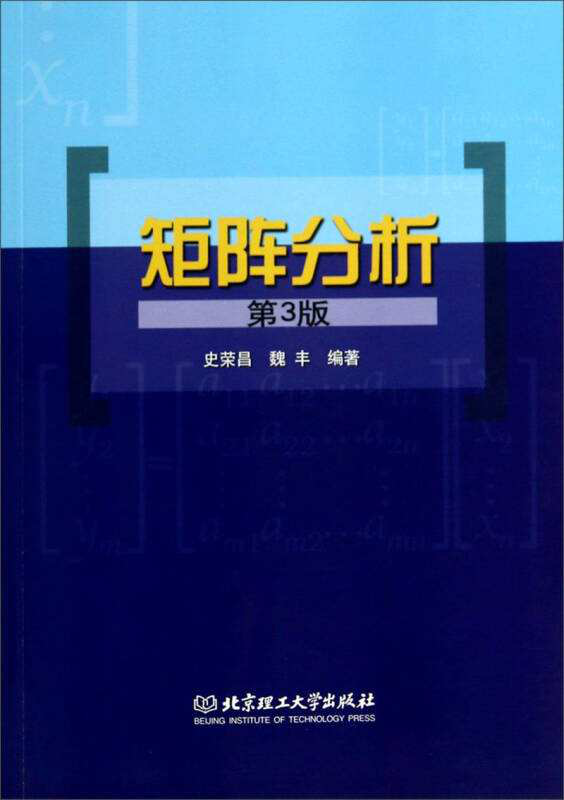
\includegraphics[scale=0.29]{book/18.png} \quad
    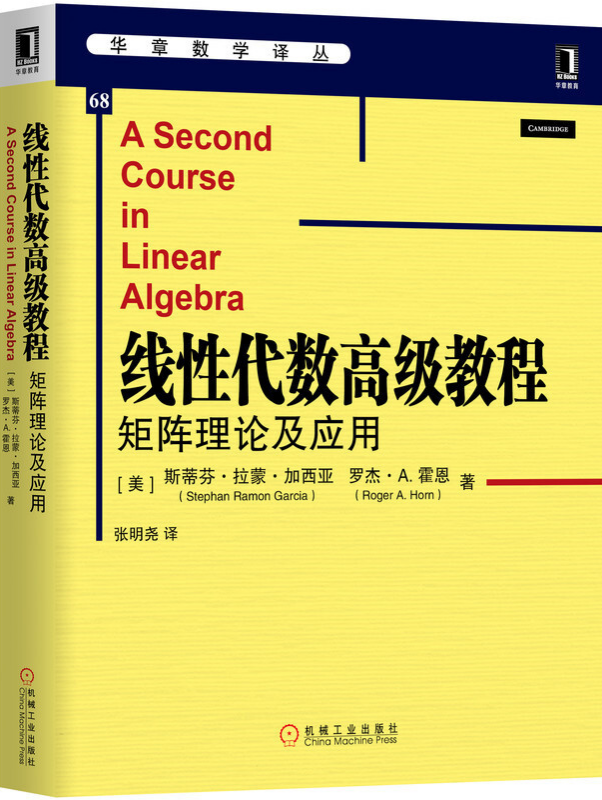
\includegraphics[scale=0.35]{book/19.png}
\end{center}

\begin{itemize}
    \item \textcite[矩阵分析]{史荣昌2010}

          这本书的内容比较偏向应用,作为动力学或控制方向的应用数学教材是很好的。这本书对于矩阵当中涉及的工具讨论的很全面,也有比较充分的计算实例,对于具备线性代数基础的同学来说自学起来也没多少障碍。

    \item \textcite[线性代数高级教程——矩阵理论及应用]{线性代数高级教程}

          这本书延续了美式教材讲解和推导详细的风格,讲解的内容全面。但同时详略比较得当,废话不多,可以作为参考。

          \begin{figure}[h]
              \centering
              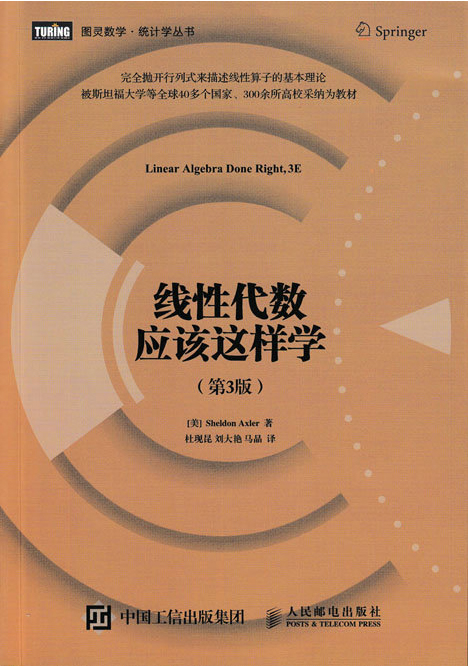
\includegraphics[scale=0.46]{book/20.png} \quad
              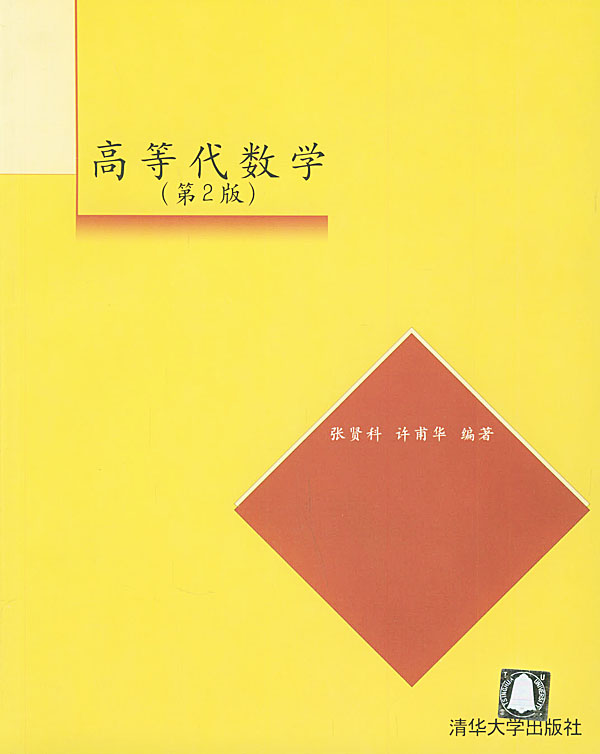
\includegraphics[scale=0.51]{book/21.png}
          \end{figure}

    \item \textcite[线性代数应该这样学]{阿克斯勒杜现昆2016线性代数应该这样学}

          这本教材的行文思路与偏向应用的参考书 \textcite[矩阵分析]{史荣昌2010} 不同,它比较侧重对线性空间和线性映射的讨论,思维上与数学专业的处理手法比较接近。由于画风接近数学专业的教材,所以该书对矩阵函数的讨论是不够的。这本教材更大的意义在于,接受了这种讨论模式后,能够更快地接受张量分析(从代数角度起讲的模式)和应用泛函分析的思路。

    \item \textcite[高等代数学]{张贤科2004高等代数学}

          这本书事实上就是数学系所使用的高等代数(对标非数学专业的线性代数,内容更多)教材之一。尽管也没有对矩阵函数做讨论,但除了矩阵分析中的内容,该书还补充了多项式理论、辛几何、张量和Hilbert空间(完备的内积空间)的内容,特别后两者分别在张量分析和应用泛函分析中都有提及,可以作为入门参考。
\end{itemize}

\paragraph{张量分析}

张量分析是力学系同学应该掌握的一项技术。如果读过徐芝纶先生所著《弹性力学》,就会感到方程的推导实在是过于繁杂和琐碎。使用张量语言的初衷,就是为了简化方程推导。

\uwave{张量}这个名词广泛的出现在物理学和力学的研究中。那什么是张量?张量事实上就是一个多重线性函数。我们在代数课程中学到线性函数可以写成向量,双线性函数可以写成矩阵,那么多重线性函数事实上也就可以写成多维数表。需要注意,这里的“维数”不是矩阵的阶数,而是指标的数量,如双线性函数对应的矩阵中的元素可以写成$a_{ij}$,那么三重线性函数对应的矩阵中的元素可以写成$b_{ijk}$,后者是没法用矩阵准确描述的。也就是说,标量、向量都可以视为特殊的张量,张量是它们的推广。

面向工科的张量课程有两种讲法,一种当然是从多重线性映射入手,这样讲更接近张量的本质,也容易进行推广,只是这种讲法对代数基础有一定要求;另一种直接从三维欧氏空间$\mathbb{R}^3$中的矢量分析讲起,可能容易上手一些,还是可以满足力学中的绝大部分公式推导需求的。

张量分析大概包括这些内容:曲线坐标系变换、张量的代数运算、曲线坐标系下张量的分析运算。学习分析部分前,可以先学习一下局部微分几何(参考书目 \textcite[微分几何]{彭家贵2002微分几何} ),这样能更快接受\uwave{指标规则},也能在学习曲线、曲面上的张量分析时容易很多。

学完张量分析,我们可以回头审视建立弹性力学、流体力学基本理论的过程,尝试用张量语言完成这一过程。另一方面,可以看一些塑性力学和连续介质力学等内容了。需要指出的是,张量语言的作用是简化复杂的运算,这是对于建立和理解理论体系、推导公式来说的,最后仍然绕不开微分方程或方程组的求解。

\paragraph{参考书目}

\begin{center}
    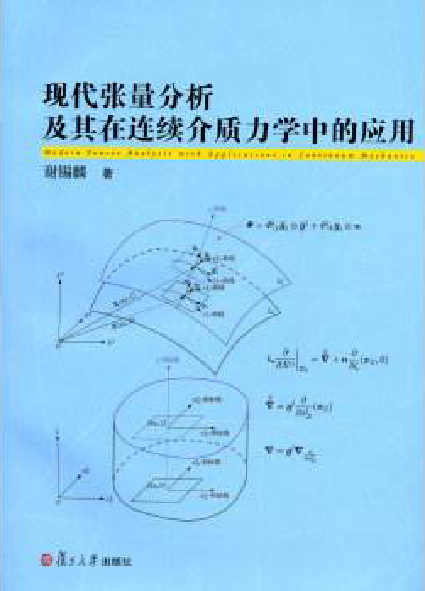
\includegraphics[scale=0.59]{book/22.png} \quad
    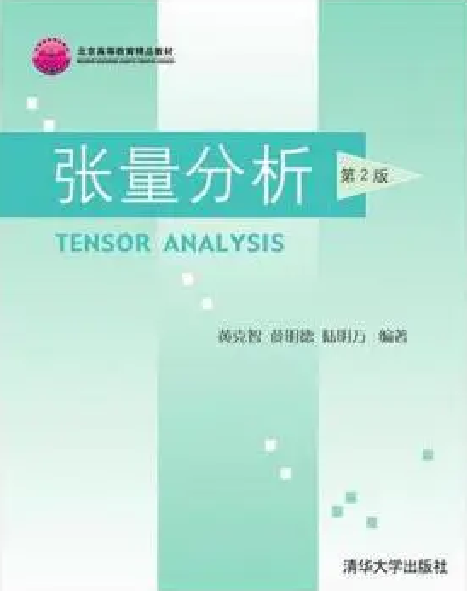
\includegraphics[scale=0.59]{book/23.png}
\end{center}

\begin{itemize}
    \item \textcite[现代张量分析及其在连续介质力学中的应用]{谢锡麟2014现代张量分析及其在连续介质力学中的应用}

          这是一本典型的从代数角度引入张量的教材。从代数角度引入张量,内容是比较全面的、逻辑也比较清晰和严谨,只是可能有一定上手难度。另外,这本书的后半段还直接对接了连续介质力学,对数学基础较好的力学系同学来说是一本不错的参考书。
    \item \textcite[张量分析]{黄克智2003张量分析}

          这本教材从分析与空间解析几何的角度引入张量,若不对张量的代数性质做太深的考虑,这本书的内容足矣。而且所讨论的张量都限制在$\mathbb{R}^3$或$\mathbb{R}^2$内,接受难度较小,也更容易直观考虑。不过该书有一点缺陷,就是第一章引入了太多运算,对于缺乏背景的同学来说可能不太容易抓到重点,所以最好有一些弹性力学的基础再看本书,可能会通畅一些。
\end{itemize}




\paragraph{偏微分方程数值解}

在后续力学课程学习与研究中,我们见到的方程多数是偏微分方程。而求解偏微分方程是十分复杂的,为了满足求解问题的需要,还是要求助于数值方法。

偏微分方程的数值格式是一个相当大的课题,而且相当多的格式都有其使用背景,所以这门课中往往也只能介绍最简单、最基本的一些数值方法。这里介绍的一般以有限差分法为主,可能会介绍一些有限元法的理论。

仍然将偏微分方程分成椭圆型、抛物型、双曲型三类讨论。在构造差分格式时,使用主要方法的仍然是Taylor展开和数值积分公式,所以在构造差分格式和误差估计这里还是容易的。椭圆型方程是这三类方程中性质较好的,在构造差分格式时基本上只需要考虑误差的问题;抛物型和双曲型方程的稳定性还与时间上的差分格式相关,所以会对这两种方程差分格式的稳定性做讨论。

构造差分格式时,有一种\uwave{有限体积法}(FVM),这种方法来自于对流体力学中守恒方程的处理,在计算流体力学、传热学等学科中的应用相当广泛,对此方向有兴趣的话可多多留意。

\uwave{有限元法}(FEM)的求解思路与最小二乘逼近有一定相似性,由于直接求微分方程的解是相当困难的,所以退而求其次,在一个给定的函数空间中寻找最接近真实解的近似解。有限元法的理论基础决定了它只能直接用在椭圆型方程上,在处理抛物型、双曲型方程时,仍然要对时间进行离散处理。有限元法中比较重要的是\uwave{Ritz法}和\uwave{Galerkin法},它们将微分方程求解问题化归成了线性方程组求解的问题。不过,由于要用到一些有关函数空间的理论,想要搞清楚有限元法的细节需要一些泛函分析的知识。

由于有限元法和有限体积法的发展比较成熟,目前这两种方法在工业界中得到广泛的应用,有相当成熟的处理具体问题的商业软件可以使用。一般来说,前边提到的数值方法在处理椭圆型方程时往往能获得不错的效果,抛物型方程次之,双曲型方程较差,这是由于双曲型方程的解中可能蕴含间断,这个间断会随着时间扩散,从而造成解的性质较差,例如反映在空气动力学上就是激波现象。

而实际问题中,往往又有不同类型方程的耦合,如抛物-双曲型方程是比较难做的(典型例子便是N-S方程),此外还有非线性方程(如描述孤立波的KdV方程)。这门课中教授的内容远远不能涵盖偏微分方程数值解的研究方向,计算数学、物理学和力学中很多问题实际上都是在做复杂方程或大规模方程的数值计算问题,学习这门课只能算是掌握数值方法的基础。近年来,为了解决实际问题,研究人员提出了许多\uwave{无网格方法},应该算是计算力学中比较热门的研究方向。



\paragraph{参考书目}\begin{center}
    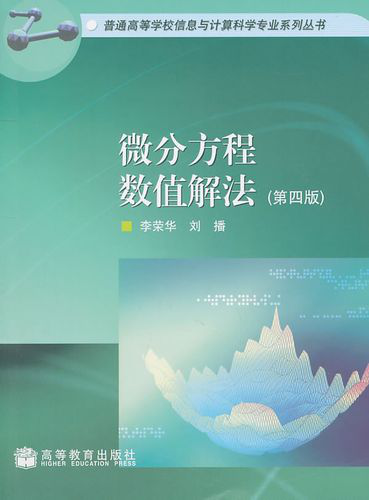
\includegraphics[scale=0.47]{book/24.png} \quad
    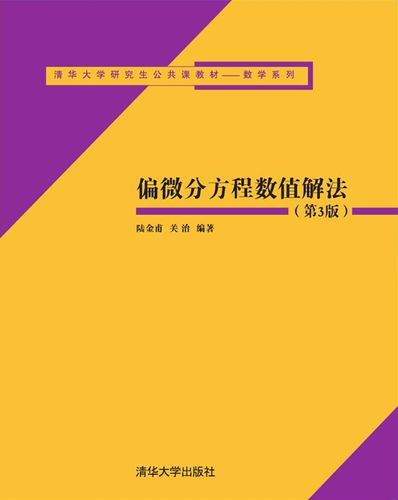
\includegraphics[scale=0.45]{book/25.png}
\end{center}

\begin{itemize}
    \item \textcite[微分方程数值解法(第四版)]{李荣华2009}
    \item \textcite[偏微分方程数值解法(第三版)]{陆金甫2016偏微分方程数值解法}
\end{itemize}

如前所述,偏微分方程数值解的课题很大,一般教材中只能覆盖最基本的内容,大体上不会差太多,这里只给出两个参考书。

\paragraph{应用泛函分析}

泛函分析研究的对象是\uwave{无穷维线性空间},由于无穷维线性空间与有限维线性空间很不一样,也不容易直观地想象出来,所以这门课大概是非数专业同学能接触到的最为抽象的基础数学课程了。

由于这门数学课比较抽象,容易遇到“学了之后不知道有什么用”的问题,所以先谈一下学习这门课的动机。泛函分析这一数学分支源自于对微分方程、积分方程求解的研究,力学专业的同学学习这门课的最终目的也正是为解微分方程服务。而为了深入研究微分方程的性质以及如何解微分方程,需要函数空间的各种理论,这就不可避免地要用到泛函分析的知识。就是说,如果要对理论有一定研究的话,泛函分析就应该是一门必修的数学基础课。然而,即使是这样比较抽象的课,学完之后可能也无法直接做什么理论性的内容,因为这门课还只是基础课,只能提供一些基本的概念和方法,想要真正提高理论水平的上限还要不断学习后续数学课程。

泛函分析是一门分析与代数并重,可能代数基础还要重要一些的数学课。有限维线性空间的研究比较容易,因为\uwave{维数是区别有限维线性空间的唯一特征},并且有限维线性空间也容易从直观上进行想象。无穷维线性空间彼此之间并不同构,并且对有限维空间的直觉在这里也可能失效,这是学习泛函分析容易遇到的另一个问题。如何解决呢?首先推导逻辑要清晰,在形成正确的“数学直觉”之前不要轻易地相信以往的经验;其次要注意从教材上的例子和从以往课程中学过的内容中寻找实例,通过足够多的例子理解概念和定理。

泛函分析这门课讨论的主要内容有:实变函数相关的基础、距离空间与赋范线性空间、内积空间以及这两种空间上线性算子的性质,此外,侧重于力学方向应用的教材可能会讲变分法与最优化的基础理论,以及Sobolev空间的基本理论。

泛函分析中要用到一些实分析的概念和定理,但对于力学系学生来说没有直接学习实分析的必要,所以在泛函分析中往往会打包一些实分析中的概念与定理以满足后续运用。在矩阵微积分部分,我们\uwave{先在有限维线性空间上引入度量,而后才能考虑其分析学性质}。这个思路在泛函分析中是一致的,但是由于无穷维线性空间与有限维线性空间中的区别,所以这里会多一些内容。无穷维线性空间中同样可以装备内积,所以也有相应的内积空间的概念。

泛函分析究竟是怎样与函数理论联系起来的呢?泛函分析讨论的是无穷维线性空间,而函数本身就能够构成一个无穷维线性空间,因此泛函分析能够处理更加抽象的函数理论。\uwave{算子}指的是一般线性空间之间的映射,当算子的“输出”是一个数域时,也称这个算子为\uwave{泛函}。赋范线性空间和内积空间上的线性算子有很多性质,这些性质是比较重要的。

引入了无穷维线性空间的度量,就能够讨论其上的分析学了。直接处理泛函的“微积分”理论就是\uwave{变分法},它是许多物理学和力学理论的数学基础,最小作用量原理说的就是泛函取极值对应一个真实物理过程,所以变分法的地位在理论推导中是很重要的。而如何求解变分问题这就涉及到函数理论了,这里便会介绍\uwave{广义函数}理论和\uwave{Sobolev空间}。

\paragraph{参考书目}

\begin{figure}[ht]
    \centering
    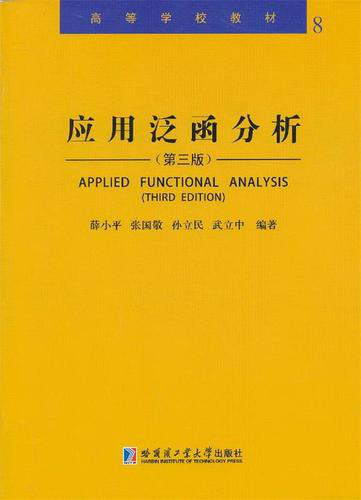
\includegraphics[scale=0.45]{book/26.png} \quad
    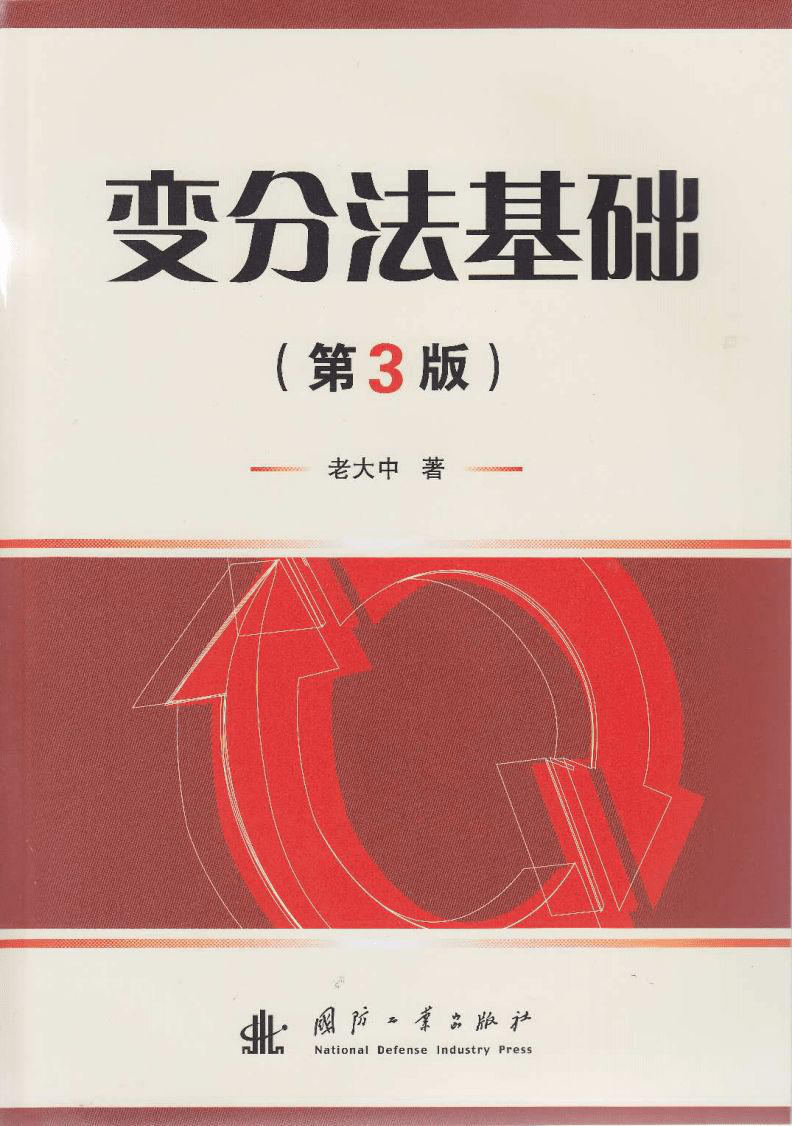
\includegraphics[scale=0.15]{book/27.png}
\end{figure}

\begin{itemize}
    \item \textcite[应用泛函分析]{薛小平2012应用泛函分析}
    \item \textcite[应用泛函分析]{柳重堪1986}     %……
    \item \textcite[变分法基础]{老大中2015变分法基础}

          这本书的起点很低,即使没有泛函分析的基础也基本能无障碍阅读,其次它不仅涵盖了各种形式的变分问题的求解方法,还补充了一些关于泛函分析的基本语言和基本知识,最后一章还讨论了变分法在力学中的应用,因此这本书对于力学的同学来说是十分好用的。
\end{itemize}
\begin{center}
    \includegraphics[scale=0.57]{book/28.png} \quad
    \includegraphics[scale=0.57]{book/29.png}
\end{center}

\begin{itemize}
    \item \textcite[数值泛函及其应用]{张维强2021}

          对于力学特别是偏工程和应用的方向来说,泛函分析很难找到其直接应用的场合,而进一步深入学习数学理论又有一定难度。这本书在泛函分析的基本理论的基础上讨论了其在数值分析中的应用,既有利于加深对数值分析的理解,也有益于对泛函分析中抽象的概念建立直观的印象。

    \item \textcite[有限元方法的数学理论]{杜其奎2012}
\end{itemize}

%……

\subsection{其他参考资料}

\begin{center}
    \includegraphics[scale=0.28]{book/30.png} \quad
    \includegraphics[scale=0.56]{book/31.png} \quad
    \includegraphics[scale=0.56]{book/32.png}
\end{center}

\begin{itemize}
    \item \textcite[力学导论]{杨卫2020}
    \item \textcite[力学史]{武际可2010}
    \item \textcite[中国力学学科史]{中国力学学会编著2012中国力学学科史}
\end{itemize}

这三本书很详细地介绍了力学的发展历史和研究现状,本手册在编写时也广泛参考了这些材料,如有兴趣,可以详细阅读这三本书。由于不可避免地涉及一些专业名词,所以在有了一定力学和数学基础后阅读这几本书的效果可能会更好。

\begin{center}
    \includegraphics[scale=0.3]{book/33.png} \quad
    \includegraphics[scale=0.56]{book/34.png}
\end{center}

\begin{itemize}
    \item \textcite[斯米尔诺夫高等数学(5卷11册)]{斯米尔诺夫2018斯米尔诺夫高等数学}

          这一系列教材是半个世纪多以前苏联使用的大学数学教材,其涵盖内容相当之广,基本上能覆盖到我们前边所讲的所有数学课程(涉及数值解的除外),而且我们也能发现部分现行数学教材参考其内容的痕迹。不夸张地说,这些书中的内容都掌握了,那么作为一名工学研究生的数学基础是十分过关的。

          该套教材分5卷:第1卷的内容大致相当于微积分;第2卷的内容大致相当于常微分方程、向量分析与场论、数学物理方程;第3卷的内容大致相当于线性代数、复变函数与保角变换、特殊函数;第4卷的内容大致是对偏微分方程做更深入的讨论,包括积分方程、变分法、偏微分方程的一般理论;第5卷的内容大致相当于实变函数与泛函分析。
    \item \textcite[数学指南:实用数学手册]{埃伯哈德·蔡德勒2012数学指南}

          这是一本十分适合与物理学研究人员和工程师使用的数学工具书。首先,内容全面而丰富,涵盖分析学、代数学、几何学、数学基础、变分法与优化、概率论与数理统计、计算数学与科学计算、数学史,能够对几乎任何学科所涉及的数学基础做查询和入门。其次,该书收录了大量的无穷级数、特殊函数、积分、积分变换等常用的表格,查询十分方便。
\end{itemize}




